\documentclass{article}
\usepackage[linesnumbered,ruled,longend]{algorithm2e}
\usepackage{amsmath, amssymb, amsthm}
\usepackage[LGR, T1]{fontenc}
\usepackage[utf8]{inputenc}   % For UTF-8 encoding
\usepackage[english]{babel}
\usepackage{csquotes} %include this when using bibLatex

\usepackage[style=numeric, backend=biber, maxnames=2, minnames=1]{biblatex}
\addbibresource{bibliography.bib} % Entries are in the bibliography.bib file


\usepackage{mathptmx} % Times New Roman font
\usepackage{multicol, relsize, geometry}
\usepackage{booktabs}
\usepackage[colorlinks=true, linkcolor=blue, urlcolor=blue, citecolor=blue]{hyperref}
\usepackage{graphicx}
\usepackage{pgfplots}
\usepackage{pgfplotstable, caption, array}
\usepackage{indentfirst}
\usepackage{setspace}
\usepackage[fracspacing]{newpxmath}
\usepackage[none]{hyphenat}
\sloppy


\singlespacing
% Adjust spacing between paragraphs
\setlength{\parskip}{1ex plus 0.5ex minus 0.2ex}
\setlength\parindent{24pt}

% Set font size and line spacing
\usepackage{setspace}
\fontsize{10}{12}\selectfont % 10pt font size with 12pt leading
\singlespacing % Ensure single spacing within paragraphs
% Needs to be last
\usepackage[table]{xcolor}

\DontPrintSemicolon
\SetKwFor{For}{for}{do}{end for}
\SetKwIF{If}{ElseIf}{Else}{if}{then}{else if}{else}{end if}%
% Redefine \ForEach to display a vertical line under it
\SetKwFor{ForEach}{for each}{}{end for}
\SetKwRepeat{Do}{do}{while}
\SetKwFor{ParallelFor}{\textbf{parallel for}}{do}{end for} % Bold keyword
\SetKwBlock{KwCritical}{\textbf{\#pragma omp critical}}{end}

\geometry{top=1cm, bottom=2cm, left=1cm, right=1cm}
\newcommand{\pluseq}{\mathrel{+}=}


\title{A heterogeneous vehicle routing problem with UAVs and multiple depots*}
\author{Panagiotis Zachos}
\date{\today}
\twocolumn
\begin{document}
	\maketitle
	\section{INTRODUCTION}
	Garnering significant academic attention since the mid-20th century, the TSP has established itself as a classic combinatorial optimization problem. In its purest form, the problem asks what is the optimal route that a salesman should take so that they can visit a set of cities exactly once and return to the origin city while traveling the minimum distance possible. This may be modeled into a graph problem by assuming a weighted undirected fully connected graph $G=\{V,E\}$ where the cities are represented by the vertices $v\in V$ and each arc $e_{v_1,v_2}\in E$ represents the distance between vertices $v_1,v_2$.
	\par
	Naturally, various generalizations have emerged to address more complex scenarios. Notably, the Vehicle Routing Problem (VRP) extends the TSP by replacing the salesman with a fleet of vehicles, each with a certain capacity, which need to service a set of customers with varying demands from a single central depot. The Multiple Traveling Salesman Problem (MTSP) lies inbetween the two previously mentioned, being an extension of the TSP and a relaxation of the VRP. In contrast to the VRP, the MTSP does not consider capacity constraints or customer demand and does not allow for multiple trips.
	\par 
	Routing problems such as the TSP and the VRP are foundational in the field of operations research and logistics as they address core issues related to efficiency, cost reduction, and resource utilization in various industries.
	Practical applications of routing problems include logistics and transportation planning, where they are used to minimize delivery times and costs; supply chain management, where they help in optimizing the distribution of products; and service industry operations, such as routing for maintenance services, garbage collection, and emergency response. One can conclude that the ability to solve these problems effectively can lead to substantial economic benefits and improved service levels across numerous sectors.
	\par 
	In recent years, the inclusion of UAVs in routing problems has gained significant attention, reflecting a growing trend towards integrating advanced technologies into logistics and operations research. This does not come as a surprise, as parcel delivery company Amazon \cite{rose2013} was first to announce their plans to use UAVs for parcel deliveries in \citeyear{rose2013}, followed soon thereafter by DHL and JD.com. Indeed, UAVs offer unique advantages by being able to bypass ground traffic and being able to reach remote or inaccessible areas.
	Regarding the last-mile delivery scenario, the underlying principle is that by making use of a lower-cost vehicle, which is also not bound by road conditions, the total time cost of operations can be reduced substantially, leading to increased efficiency and thus profitability for the distributor but also increased customer satisfaction and reduced environmental footprint. By adding UAV(s) alongside traditional vehicles, the distance that the latter need to travel is reduced, leading to overall cost reduction of the operation (fuel consumption, working hours) while simultaneously limiting CO2 emissions.
	Apart from delivery services, the use of UAVs introduces new dimensions to the traditional routing problems by offering innovative solutions for surveillance and inspection tasks such as in agriculture, where UAVs may be used for crop monitoring and spraying. Another practical application benefitting from the use of this technology is disaster response, where their agility may provide rapid assessment and delivery of critical supplies.
	\par
	Although a rich amount of research has emerged in recent years regarding routing problems that are concerned with incorporating UAVs alongside traditional last-mile delivery means (trucks), to the best of our knowledge we are the first to consider a heterogeneous fleet of road vehicles along with independent UAV operations and multiple depots. Considering that companies active in the parcel delivery industry in Greece make use of motorbikes (scooters) in last-mile delivery and in the case of large cities there are multiple last-mile shops operating from where the vehicles are loaded to service customers,
	(our study depicts a real-world scenario/we study a scenario with real-world applications). We propose a fast heuristic and a more computationally demanding hybrid Ant Colony Optimization metaheuristic that is able to yield better solutions.
	\par
	
	\section{Related Work}
	\citeauthor{Murray2015} \cite{Murray2015} were the first researchers who formalized and extensively studied the concept of UAVs working alongside trucks in routing problems in 2015. In their seminal paper they introduced the Flying Sidekick Traveling Salesman Problem (FSTSP) and the Parallel Drone Scheduling Traveling Salesman Problem (PDSTSP). The two problems are similar in their use of a single truck alongside one or more UAVs but there are key differences between the two.
	\par
	\subsection{The Flying Sidekick Traveling Salesman Problem} 
	The FSTSP involves a truck with unlimited capacity which takes on the role of the salesman, and is equipped with a single UAV (drone) which the driver can utilize by dispatching it to serve drone-eligible customers. The objective is to minimize the total time in which all customers are serviced.
	In the FSTSP a truck and a drone are called to begin from a depot, although not necessarily in tandem, visit a set of customers exactly once, and then end their tour by returning to the depot. The driver is considered to load the UAV with the parcel of the intended customer inbetween traveling i.e when the truck has stopped at a customer location to deliver a parcel. Then, the driver dispatches the UAV and immediately continues with the truck onto the next customer(s), thus creating a time window in which both the truck and UAV are traveling simultaneously. After the UAV has delivered its parcel, it must return to the truck to be retrieved by the driver, or if flight endurance limitations allow, it can return to the depot, thus ending its tour. The retrieval of the UAV by the truck must be performed at a customer location assigned to the truck, which must be different from the launch location i.e the truck cannot remain stationary after launching the drone. The vehicle which arrives first at the determined retrieval node has to wait for the other vehicle, therefore synchronization between the truck and drone is required. Furthermore, the drone is associated with a launch setup and a retrieval time cost which must be considered in the synchronization and a maximum flight endurance value (battery capacity) which must be respected when assigning customers to the drone.
	\par
	The authors used MILP to model the problem and noted that, deriving from the NP-hard nature of the problem, MILP solvers in certain cases required several hours even for instances with as low as 10 customers. Consequently, they proposed a route and re-assign heuristic. The heuristic begins by solving a TSP that assigns the truck to visit all customers. This TSP subproblem was solved using various techniques, namely Integer Programming (IP), and the \citeauthor{CW1964} Savings \cite{CW1964}, Nearest Neighbour, Sweep heuristics. Once the truck route is established, the heuristic attempts to improve the solution by re-assigning customers to the drone. The algorithm iterates through each pair of consecutive stops in the truck route and for each pair considers the possibility of sending the drone from the first stop to the second stop. Next, the savings in travel time that would result from making this change are calculated, while considering the drone's and truck's travel time as well as the time required to retrieve the drone. If the resulting savings are greater than zero, the customer at the second stop is re-assigned to the drone and the truck route is updated accordingly. The heuristic continues to iterate through all pairs of stops in the truck route, re-assigning customers to the drone whenever possible, until no further improvements can be made. 
	\par
	\citeauthor*{Ha2015} \cite{Ha2015} researched the FSTSP, although under a different name; the "Traveling Salesman Problem with Drone". They proposed two heuristics using two opposite concepts; (i) cluster first - route second and (ii) route first - cluster second. The clustering step consists of determining the set of drone routes that should be in the final solution. To solve this, the authors propose a Mixed Integer Linear Programming (MILP) model where the objective function is to maximize the profit generated by selecting specific drone routes. 
	In the first approach, the MILP model is initially solved, to identify the optimal set of drone routes. Once those are determined, the heuristic then constructs the truck's route, using the Concorde TSP solver \parencite{ConcordeTSP}, by integrating the drone's routes with the remaining customer locations, producing the final solution. In the second route first - cluster second approach, the truck route is first solved, visiting all customers. The truck's route is then used as the basis to identify potential drone routes. The MILP model used in the clustering step is adapted to include constraints that ensure that any drone route selected is part of the truck's predetermined tour and that the nodes that form the drone \textit{sortie} are arranged in the same order as they appear in the truck's route.
	\par
	In \cite{DeFreitas2018} \citeauthor{DeFreitas2018} extended the FSTSP research and employed a hybrid heuristic termed Randomized Variable Neighborhood Descent Framework (RVNDF) to solve the problem. This heuristic makes use of a three-step approach. The RVNDF begins by generating the optimal solution for the TSP where all of the customers are serviced by the truck only, using the Concorde TSP solver. The second phase consists of creating an initial solution which makes use of the drone, by assigning it to random drone-eligible customers while respecting the drone's flight endurance. Finally, in the third step, the Randomized Variable Neighborhood Descent algorithm is called, a VND algorithm where the order of the neighborhood visits is not predetermined. This randomized local search procedure aims to improve the initial solution by systematically exploring different neighboring solutions. It does this by applying five different "neighborhoods" or local search operations, each designed to modify the current solution in a specific way. These neighborhoods consist of the following 5 operations: (i) \textit{Reinsertion}: Moving a truck customer to a different position on its route, (ii) \textit{Exchange}: Swap the positions of two truck customers, (iii) \textit{Exchange(2,1)}: Swap the positions of two consecutive customers and  an other one, (iv) \textit{2-Opt}: Remove two non-adjacent arcs from the truck's route and insert two new arcs such as to create a new route, (v) \textit{RelocateCustomer}: Transfer a customer from the truck's route to the drone's route. The RVNDF evaluates all possible moves within each neighborhood, ensuring that the drone's flight range and customer accessibility constraints are respected. After each operation, the resulting solution is either accepted and used to update the current solution if the overall delivery time improves, or discarded otherwise.
	\par
	\{REMOVE\}
	\citeauthor{DellAmico2019} \cite{DellAmico2019} proposed a modified formulation of \citeauthor{Murray2015}'s FSTSP, aiming to improve it and achieve a more realistic interpretation of the problem. They considered two different versions, one where the drone is allowed to land and wait at customers to conserve battery and another where waiting is only allowed in flight. The authors also introduce a three-indexed formulation termed DMN and a two-indexed formulation DMN2. The objective function aims to minimize the overall completion time, accounting for the truck's travel time, drone launch and return times, and waiting time at customers if applicable.
	The DMN formulation leverages three-indexed boolean variables to represent \textit{sorties}; flights undertaken by the drone. This formulation includes various improvements which are focused on eliminating infeasible drone sorties. To achieve this, a new objective function and a set of inequalities are presented.
	The two-indexed formulation, DMN2, simplifies the representation of sorties by using two-indexed arc variables. These variables represent the drone's entry and exit points from customer nodes. This approach significantly reduces the number of variables needed, leading to a more efficient and faster solution process. DMN2 is built upon the DMN formulation, adapting all constraints involving the three-indexed variables to use the new two-indexed variables. The objective function in DMN2 is also modified to reflect the use of two-indexed variables. Due to their exponentially large number of constraints, these models required a branch-and-cut implementation.
	\par
	\{REMOVE\}
	In a subsequent paper \cite{DellAmico2021}, the same authors proposed two algorithms to solve the FSTSP; a Branch and Bound (BB) algorithm and a heuristic based on the aforementioned for larger instances. The BB algorithm utilizes the concept of "missions" which can be either truck movements or phases where the truck and drone operate in parallel. It works by incrementally expanding partial solutions by adding new missions at each level of the search tree until the final depot is reached. Customers are assigned to drones only in the final stage by solving an Assignment Problem \cite{AssignmentProblemSurvey2006}, a strategy aimed at limiting the search tree size. The heuristic, heavily based on BB, begins with an initial feasible TSP solution and then repeatedly applies the BB method as a subroutine, iteratively refining the solution by adding drone services to optimize the overall delivery time.
	\par
	\citeauthor{Boccia2021} \cite{Boccia2021} proposed compact integer linear programming formulations for the FSTSP, making use of a novel extended graph representation avoiding the use of big-M constraints, a common drawback of existing models. The authors approach the problem by leveraging a Branch-and-Cut (B\&C) algorithm coupled with a column generation procedure \cite{ColumnRow1960}. The B\&C procedure begins by considering a subset of variables and constraints and progressively adds more complex ones as needed. The column generation procedure avoids a full enumeration of variables, leading to more efficient computation.
	\par
	Genetic algorithms also have been proposed in recent years to solve the FSTSP. \citeauthor{Kuroswiski2023} \cite{Kuroswiski2023} presented an improved MILP formulation and a Hybrid Genetic Algorithm (HGenFS). The formulation, based on existing work, significantly reduces the complexity of the original model with 28 restrictions to just 13 constraints.
 	The HGenFS algorithm utilizes a chromosome representation that incorporates both the sequence of deliveries and the delivery method (truck or drone) for each customer. The algorithm employs a number of optimization techniques, including:  (i) \textit{Crossover}; two crossover methods, for combining information from parent chromosomes to generate offspring, (ii) \textit{Mutation}; two mutation methods to diversify the population, including swapping customer positions and alternating the delivery method, (iii) \textit{Local Search}; a local search phase to further refine the solution, exploring alternative drone routes and delivery methods.
	\par
	\citeauthor{Pilcher2023} \cite{Pilcher2023} proposed a novel self-adaptive genetic algorithm (GA) with a novel two-stage mutation process designed to address the complexities of the FSTSP. This GA distinguishes itself by co-evolving a memeplex alongside the population, where the memeplex comprises eight options representing crossover and mutation operators and their probabilities of being applied. This dynamic adaptation of the algorithm enables it to learn and adjust its evolutionary strategy over generations. Additionally, the newly proposed two-stage mutation process allows for simultaneous modifications to the tour sequence and node types within a single generation, offering greater flexibility in exploring the search space. The algorithm also incorporates a range of problem-specific crossover and mutation operators, dealing with swapping customer nodes to different places in the tour or swapping customers between vehicles. Furthermore, the initial population generation leverages a scoring system based on potential makespan savings, encouraging exploration of non-obvious drone node configurations.
	
	\subsection{The Parallel Drone Scheduling Traveling Salesman Problem}
	The PDSTSP, introduced in the same paper \cite{Murray2015} by \citeauthor{Murray2015}, alters the concept of the FSTSP by involving multiple drones and optimizing the delivery process through parallel drone operations. In contrast to the FSTSP, the drones act independently from the truck and launch from and return to the depot. It was designed for scenarios where a significant portion of the customers are located within the UAV's flight range from the depot. This problem can be reduced to two classic, widely researched operations research problems, the TSP; to find the optimal truck route, and the Parallel identical-Machines Scheduling problem (PMS); to find the optimal assignment of UAVs (machines) to customers (jobs), such that the total completion time (makespan) of the UAV fleet is minimized. The authors proposed a MILP formulation and employed heuristic algorithms to solve larger instances of the PDSTSP.
	The heuristic proposed by the authors is a greedy, iterative approach that aims to partition customers between the truck and the UAV fleet. The heuristic begins by assuming all UAV-eligible customers are assigned to the UAV fleet and the remaining customers are assigned to the truck. Regarding the latter, a TSP route is solved using three methods; \textit{(i) MILP}, \textit{(ii) Savings heuristic}, \textit{(iii) Nearest Neighbour heuristic}. To solve the PMS and optimally assign the UAV fleet to customers, a binary integer programming (IP) formulation and the Longest Processing Time first (LPT) heuristic were used. This initial assignment is then refined iteratively by re-assigning individual customers between the truck and UAV partitions. The heuristic calculates the total completion time for the UAV fleet and for the truck route based on their respective assignments. It then aims to balance the total makespan by re-assigning customers. If the UAV makespan exceeds the completion time of the truck route, the heuristic seeks to reduce the UAV makespan by transferring a customer from the UAV partition to the truck partition. In the same manner, if the truck's route exceeds the UAV makespan, it attempts to find the best customer node to be swapped from the truck to the UAV partition. The algorithm chooses the move that offers the greatest net savings in overall makespan via use of the LPT algorithm. This process of reallocating customers continues until no further improvements can be made.
	\par
	\citeauthor{MbiadouSaleu2018} \cite{MbiadouSaleu2018} proposed an MILP formulation along with an iterative two-step heuristic. First, a coding step transforms a given PDSTSP solution into a customer sequence, representing the order in which customers are visited. Next, a decoding step decomposes the customer sequence into a tour for the vehicle and sorties (trips) for the drones. This decoding step is formulated as a bicriteria shortest path problem \cite{biCriteriaSP} and is solved using a dynamic programming approach which involves progressively associating a list of labels with each node in the graph representing the customer sequence. Each label represents the cost vector of a partial path, calculated by summing the costs of the currently crossed arcs. These label lists are iteratively built, employing bounding mechanisms and a dominance rule to reduce the computational complexity. The authors also address the challenge of handling multiple drones (M > 1) by adapting the decoding procedure and introduce an approximation where the drone delivery time is shared equally among the drones, allowing them to utilize the same dynamic programming scheme as in the single-drone case.
	\par 
	\citeauthor{Dinh2021} \cite{Dinh2021} propose a Hybrid Ant Colony Optimization (HACO) algorithm to solve the problem. This algorithm is built on the idea of representing the PDSTSP as a giant TSP tour, which is then decomposed into a truck tour and drone sorties using a dynamic programming approach. This approach considers the time cost of both the truck and the drones, and aims to balance the workload such as to minimize the overall completion time of the operation. To further enhance the efficiency and quality of the algorithm, the authors incorporate several components adapted from other metaheuristics, such as a drone node selection step based on Large Neighborhood Search, and a 3-opt local search for improving the TSP tour.
	\par
	In \cite{MbiadouSaleu2022} Mbiadou Saleu at al. introduce the Parallel Drone Scheduling Multiple Traveling Salesman Problem (PDSMTSP), where a fleet of both trucks and drones operating independently are tasked with delivering packages to customers. The objective remains that same as the PDSTSP; minimization of the overall delivery completion time. The authors propose a hybrid metaheuristic algorithm to solve the PDSMTSP, building upon their previous work for the single-truck case. The algorithm begins by constructing a giant tour, considering only one truck that visits every single customer using Nearest Neighbor. Then, a dynamic programming procedure, named "split", decomposes the giant tour into complementary subsequences, assigning customers to a different truck or to the set of customers serviced by drones. This procedure is implemented by considering an acyclic directed graph and solving a multi-criteria shortest path problem.
	Each vehicle route is then reoptimized using the TSP Lin-Kernighan \cite{Lin-Kernighan2000} heuristic to obtain optimal or near-optimal routes for the vehicles. Customers assigned to drones are allocated to individual drones using the Longest Processing Time first (LPT) heuristic, solving a Parallel Machine Scheduling (PMS) problem. Finally, a local search procedure consisting of various moves is called to improve the constructed tours of the current solution by swapping customers between the trucks or between trucks and drones. At the end of each generation, the resulting solution is compared to the best solution found so far and is updated if better.
	\par
	\citeauthor{Montemanni2023} \cite{Montemanni2023} proposed a novel Constraint Programming model for the PDSTSP which leverages recent developments in black-box solvers \cite{Black-BoxSolvers} capable of exploiting parallel computation. This approach provides a novel perspective for optimization on modern personal computers, offering a compelling alternative to traditional heuristic methods that often struggle with large instances. The model utilizes a set of binary variables to represent the truck's tour and the drone assignments, respectively. Additionally, an additional variable captures the objective function value, representing the time taken by the last vehicle to return to the depot.
	\par
	%%%%%%%
	\subsection{TSP-D}
	\citeauthor{Agatz2018} \cite{Agatz2018} introduced the Travelling Salesman Problem with Drones (TSP-D). While the TSP-D shares mostly the same characteristics as the FSTSP, the authors decide to neglect the delivery time cost of both vehicles and the recharging time cost of the drone. The authors model the problem and propose an IP formulation with which they manage to solve instances with up to 12 customers to optimality. As exact methods become computationally intractable for larger instances, the authors propose several fast route first-cluster second heuristics based on local search and dynamic programming. These heuristics first construct a truck-only TSP tour using either an optimal TSP solution (Concorde) or the faster minimum spanning tree (MST) algorithm \cite{MST1957}. Next, they assign drone nodes to this tour using either a fast greedy partitioning heuristic or an exact partitioning algorithm where a dynamic programming algorithm is employed to find an optimal partitioning of the TSP tour into truck and drone subtours. 
	To refine the solution, the authors apply an iterative improvement procedure that modifies the initial TSP tour and re-evaluates the drone node assignment using the chosen partitioning method. The authors provide a theoretical analysis of their heuristics, establishing a worst-case approximation guarantee for their heuristics, and demonstrating their effectiveness in providing near-optimal solutions. They also prove a lower bound on the optimal solution value of the TSP-D, showcasing that TSP algorithms can be used as approximation algorithms for the TSP-D.
	\par
	\citeauthor{Yurek2018} \cite{Yurek2018} contributed to the TSP-D research by proposing a decomposition-based, two-stage iterative optimization algorithm. In the first stage, the truck route is determined by generating all of the possible truck routes, considering only customers that are not drone-eligible, and keeping those whose route duration is shorter than the global  upper bound (gub) which is initially set by the TSP solution of the problem. These eligible truck routes then pass onto the second stage where a MIP formulation is solved to determine the optimal drone routes for the remaining customers. After the final TSP-D solutions have been constructed, the best one is kept and it replaces the current gub if it is better (shorter) than the current. To improve the efficiency of the algorithm, the authors propose a heuristic to significantly reduce the number of truck routes generated in the first stage. This heuristic utilizes the nearest neighborhood approach for each possible drone node assignment, generating a single truck route and eliminating other routes involving the same customer nodes in different sequences.
	\par
	\citeauthor{Ha2018} \cite{Ha2018} introduced the min-cost TSP-D, a novel variant of the problem with the objective of minimizing the operational costs, which include transportation costs and waiting penalties for both the truck and drone. The authors proposed a MILP formulation and two heuristic methods to solve the problem. The TSP-LS heuristic, adapted from the heuristic by \citeauthor{Murray2015}, is designed to solve the min-cost TSP-D problem by converting an optimal TSP solution into a feasible TSP-D solution through a series of local searches. It begins by calculating cost savings for relocating a truck node to a different position or inserting a drone node between two existing nodes in the truck tour. Based on these cost savings, the algorithm then iteratively relocates truck nodes and inserts drone nodes, seeking to improve the solution, and terminates when no further positive cost savings can be achieved. The second proposed heuristic is a Greedy Randomized Adaptive Search Procedure (GRASP) that aims to solve the problem. First, the construction phase involves a split algorithm that converts a TSP solution into a feasible TSP-D solution. This is achieved by building an auxiliary graph where each subsequence of nodes represents a potential drone delivery and then extracting the shortest path in the graph which corresponds to the best TSP-D solution derived from the initial TSP tour. The local search phase further improves the constructed solution through a set of operators, including relocation, drone relocation, and drone removal. The authors also adapt the GRASP algorithm to address the min-time TSP-D problem by adjusting the cost computation in the auxiliary graph to prioritize time over cost.
	\par
	\subsection{Other}
	\{ADDED\}
	 \citeauthor{Lu2022} \cite{Lu2022} suggest a unique model coined the Flexible Drones Traveling Salesman Problem (FDTSP), in which a truck serving as a parcel delivery vehicle but also as a mobile launch platform for several drones, is tasked with finding the optimal route such as to deliver packages to customers within specified time slots. The authors propose a two-phase heuristic method. Initially, customers are grouped according to time slots and location using a bisecting K-means algorithm. The customer nodes are iteratively divided into clusters, ensuring that the number of customer nodes in each cluster does not exceed the combined number of drones plus the truck. Then, the centroid of each cluster is identified and the customer node nearest to it is selected as the one to be visited by the truck, while the rest are left for the drones. In the second phase, the goal is to discover the quickest truck route connecting all of the clusters based on the nodes selected in the previous step. Three metaheuristic techniques are examined: OR-Tools, Genetic Algorithm, and Simulated Annealing. Once the truck route is established, the drones are deployed to serve the customers within their respective clusters, respecting their battery endurance constraint. After a drone has completed a delivery, it returns to the truck in the next cluster, allowing it to be readied for subsequent deliveries. Naturally, there are occurences where this is not possible due to battery limitations. The authors propose two solutions for when such cases arise. The first sees the drones returning to the truck in the same cluster, resulting in the truck spending extra time waiting for them. The second proposition regards cases where the drones are unable to even reach the customer, thus leading to the truck taking them on, which in turn necessitates a re-optimization of its route.
	 \par
	%
%	\subsection{The Vehicle Routing Problem}
%	The Vehicle Routing Problem (VRP) is a cornerstone in the field of combinatorial optimization and logistics, focusing on the optimal routing of a fleet of vehicles to service a set of customers. Since its introduction by \citeauthor{VRP1959} in 1959 \cite{VRP1959}, numerous variants and extensions of the VRP have been developed to address practical and complex logistics challenges. These include considerations for time windows, multiple depots, and heterogeneous fleets, each adding layers of complexity to the original problem. The VRP in its original form seeks to determine the optimal set of routes for a fleet of vehicles located in a single depot node to deliver goods to a set of customers, minimizing the total cost while satisfying constraints such as vehicle capacity and customer demand. The cost is typically defined as either the total distance, time, fuel consumption, pollution or a combination of those. The primary distinction between the VRP and the TSP lies in the capacity constraint of the vehicles and the product demand of the customers; the vehicles return to the depot when they can no longer service any customer, to either reload or finish their tour. When the vehicles have unlimited or sufficiently large capacity as to not restrict their movement, the CVRP effectively reduces to a multiple Traveling Salesman Problem (mTSP).
%	\par
%	The rapid advancement of drone technology has spurred significant interest in its application to logistics and transportation, particularly in addressing the complexities of last-mile delivery. Vehicle Routing Problems with Drones (VRP-D) represent an innovative extension of traditional VRPs, where drones are deployed alongside traditional delivery vehicles to enhance efficiency and reduce operational costs. This integration leverages the agility and speed of drones to complement the capacity and range of trucks, presenting new challenges and opportunities in route optimization. The VRP-D and its variants focus on optimizing the coordinated routes of both vehicles and drones to ensure timely and cost-effective deliveries, considering constraints such as drone battery life, payload capacity, and synchronization requirements. This literature review explores the foundational concepts of VRP with Drones, the evolution of algorithmic approaches, and the diverse applications and implications of integrating drones into vehicle routing problems.
%	\par 
	%
	\subsection{The Vehicle Routing Problem with Drones}
	\citeauthor{Wang2017} \cite{Wang2017} introduced the Vehicle Routing Problem with Drones (VRPD), where a fleet of $m$ trucks, each capable of carrying a number $k$ of drones, deliver packages to customers with a demand of 1 parcel each. The primary objective is to minimize the total completion time in which all of the customers are serviced. Each drone must be launched and recovered from the same truck and synchronization between the two is needed, but unlike the FSTSP and TSP-D, the authors allow the drone to launch from and return to its truck at the same node location. Furthermore, the authors assume a drone battery large/efficient enough such that it does not limit the drone's flight endurance and the drone capacity to be equal to 1 parcel i.e drones can service one customer per sortie, while trucks have a capacity $C$, and both the truck and drone follow the same road network. To address the VRPD the authors employ a worst-case analysis approach to evaluate the potential benefits of integrating drones into the vehicle routing problem. This analysis is structured around comparing the traditional VRP, which utilizes trucks only, to the VRPD. The authors establish theoritical bounds on the time savings achievable by formulating several theorems that derive upper bounds on the ratio of the completion times of these two problems, aiming to demonstrate that the use of drones can lead to significant reductions in delivery times.
	\par 
	\citeauthor{Schermer2018} \cite{Schermer2018} address a modified version of the above VRPD. In this paper, the authors assume that the drones have a limited flight range due to battery capacity and that they cannot be recovered at the same node location where they were launched from. The authors introduce a Two-Phase Heuristic (TPH) and a Single-Phase Heuristic (SPH) to solve the problem. The TPH begins by constructing a VRP tour using the Nearest Neighbor heuristic. This initial tour includes all customer vertices and is then split into segments corresponding to the number of available $m$ trucks. In the first phase, the algorithm focuses on improving the VRP solution by employing improvement techniques such as 2-opt local search and \textit{String Mix} (SM): a combination of \textit{String Exchange} which exchanges two random customers between two tours and \textit{String Relocation} which relocates a node to a different tour. After a predetermined amount of time has passed, the algorithm enters the second phase, where drones are integrated into the constructed routes. This involves two procedures: \textit{Drone Insertion} (DI); drones are inserted into the existing tours based on the first feasible sortie that reduces the overall completion time and \textit{Delivery Exchange} (DE); attempts to change the delivery method of one tour between the truck and the drone, ensuring that the time to complete the tour is minimized. Similarly, the SPH starts with the NN heuristic to create an initial tour that includes all vertices. Unlike the former, the SPH inserts drones into the routing solution right after the initial tour is created. This means that the drone operations are considered throughout the entire optimization process along with the truck operations, and the algorithm iteratively calls the aforementioned optimization procedures (2-opt, SM, DI, DE) until a stopping criterion is met.
	\par 
	%The same authors in \cite{Schermer2019} introduced for the first time a MILP formulation for the VRPD which supports multiple drones per truck and cyclic drone operations (drones may return to the same node they were launched from). To enhance the performance of MILP solvers, the authors propose several sets of valid inequalities that significantly improve the solver's ability to find optimal solutions for small instances. However, acknowledging the limitations of MILP formulations for larger instances, they also develop a matheuristic to solve the problem. This matheuristic effectively exploits the problem structure of the VRPD and incorporates the proposed \textit{Drone Assignment and Scheduling Problem} (DASP) as a key component, which aims to optimize the assignment and scheduling of drones based on existing truck routes.
	%\par
	\citeauthor{Sacramento2019} \cite{Sacramento2019} expanded the research by introducing additional constraints to further simulate real-world challenges. The authors take into account time constraints associated with the launch and recovery of the drone, service times for customer deliveries, limited truck capacity and a truck maximum route duration. In the VRP-D proposed, a fleet of homogenous trucks, each equipped with a single drone must service a set of customers with known demands while minimizing the total operational cost. This cost is defined as the sum of the transportation costs incurred by both the trucks and the drones. Specifically, the cost for the truck is related to the fuel price and consumption rate, while the cost for the drone is set as a factor of the truck's cost, reflecting that using the UAV is considerably cheaper than using the truck. The authors propose a mathematical model that extends the Mixed Integer Programming (MIP) formulation of the FSTSP, incorporating multiple trucks and capacity and time constraints. To solve the problem, the authors employ an Adaptive Large Neighborhood Search (ALNS) metaheuristic. This algorithm iteratively enhances an initial solution by utilizing a systematic approach that combines destruction and repair methods. The initial solution is generated through a three-phase process. First, the Nearest Neighbor heuristic is used to obtain a truck-only solution. Then, a String Relocation local search algorithm is employed to refine the truck-only solution. Finally, a drone addition algorithm is called which considers all drone-eligible customers to be swapped from the truck to the drone, and iteratively makes swaps that provide the maximum possible savings until no improvement is possible. The ALNS operates by first destroying a portion of the current solution, allowing for exploration of new solution spaces, with the destruction controlled by parameters that determine the number of customers to remove. The algorithm adapts the choice of destruction and repair methods based on their historical performance, facilitating dynamic search processes that can escape local optima. The ALNS incorporates an acceptance criterion inspired by Simulated Annealing, permitting the acceptance of worse solutions with a certain probability, particularly in the early search stages.
	\par 
	%\citeauthor{Wang2019} \cite{Wang2019} propose a novel arc-based MIP model along with a branch-and-price algorithm to solve the VRPD. Due to the complexity and large number of constraints in their model, the authors reformulate the problem into a path-based model, focusing on feasible paths for both trucks and drones, allowing for a more efficient solution process. Then, the authors introduce a branch-and-price algorithm which consists of three key components. First, a pricing sub-problem which aims to find the minimum reduced cost paths for both trucks and drones. The authors design a specialized network that distinguishes between different types of paths and nodes, facilitating the identification of optimal routes. Next, the algorithm employs column generation \textbf{\{RESEARCH\}} techniques to manage the large number of potential paths efficiently. This involves generating new columns (paths) iteratively based on variables from the restricted master problem. Finally, to mitigate slow convergence issues, the authors implement stabilization techniques, including the computation of alternative Lagrangian lower bounds and the application of column generation stabilization methods.
	%\par 
	\citeauthor{Lei2022} \cite{Lei2022} address the VRPD as formulated by the previous authors by proposing a Dynamic Artificial Bee Colony (DABC) algorithm, which solves the problem by dynamically managing two swarms of artificial bees - employed bees and onlooker bees. Following the Artificial Bee Colony (ABC) principles, employed bees have the role of recognizing the nectar amount of a food source and thus indicating the fitness of a move to the onlooker bees, which then choose appropriately their next move.
	Initially, the algorithm produces two bee swarms, with each containing a set of solutions obtained using four different heuristics: (i) Savings \cite{CW1964}, (ii) Sweep \cite{Sweep1974}, (iii) Cheapest insertion \cite{CheapestInsertion1976} and (iv) Nearest Neighbor. The algorithm works by iteratively evaluating these swarms to determine which should be named the employed bee group (EB) and which the onlooker bee group (OB). In each generation, a comparison process first evaluates the solutions in each swarm and the role of EB is given to the swarm with the best solutions while the other is named OB.
	The algorithm continues by entering the employed bee phase where the solutions in the EB swarm undergo a Variable Neighborhood Descent (VND) process which consists of fifteen neighborhood structures. Next, in the onlooker phase, solutions in the OB swarm are assessed against the average objective value of the group, and if a solution is below this average, it is also subjected to VND; otherwise, a probabilistic decision is made to either perform VND or replace the solution with one from EB through a binary tournament. The DABC also incorporates a scout phase, where solutions that fail to improve after a set number of trials are replaced with new random solutions. The above take place in a sequential iterative manner until the algorithm's stopping condition is met.
	\par 
	\citeauthor{Stodola2024} \cite{Stodola2024} were the first to research the multi-depot concept in routing problems with drones, using the term MDVRP-D. The authors introduced a mathematical formulation and proposed an Ant Colony Optimization (ACO) algorithm to efficiently solve instances of the problem. More specifically, the authors expand on their previous work on the Multi-Depot Vehicle Routing Problem \cite{Stodola2022}, for which they have proposed the Adaptive Ant Colony Optimization with Node Clustering (AACONC) algorithm, by adding drones to the equation. In the MDVRP-D, each depot is equipped with 1 or more trucks, each of which is equipped with 1 drone, similar to the FSTSP. They study two objective functions, minimizing the total completion time of the operation and minimizing the total cost of the operation. The principle of Ant Colony Optimization involves simulating the behavior of ant colonies searching for optimal paths between an ant nest and food sources using pheromone trails. In this context, ants represent the trucks equipped with drones and pheromone trails represent the attractiveness or optimality of a particular route. To adapt for the use of drones, two pheromone matrices are used; one for the trucks and an additional one for the drones. The algorithm begins by initializing these matrices and proceeds by creating clusters of transition vertices for each vertex in the graph, using the \textit{node clustering} principle \cite{Stodola2020} to group vertices based on their probability of belonging to the optimal solution. The algorithm then iteratively generates ant solutions, each representing a potential route configuration for trucks and drones. Each ant solution is constructed iteratively, probabilistically selecting the next node (customer) to be serviced based on the pheromone matrices; First, it probabilistically selects a depot based on pheromone potential. It then builds routes by using a two-phase approach: selecting a cluster based on pheromone trails and then choosing a customer within the cluster. During this route construction, the algorithm also makes probabilistic decisions to dispatch drones based on the strength of pheromone trails associated with candidate customers. If a drone is dispatched, the algorithm utilizes the node clustering principle again to select a customer within a cluster for the drone to service. After a set amount of ant solutions have been produced, the best one of this generation is kept while the others are discarded. Periodically, the algorithm performs local search optimization on this solution, adjusting the routes of trucks and drones to further improve the solution quality. This optimization phase involves exchanging customers between truck routes and drone routes, as well as adjusting the launch and recovery points of drone sorties to enhance their efficiency. At the end of each ant generation, the algorithm updates the pheromone matrices based on the quality of the generated ant solutions, employing the simulated annealing principle and an adaptive pheromone evaporation procedure to prevent convergence on local optima. The algorithm terminates either when a predetermined amount of generations have passed or when the diversity of the population of the solution set approaches its lower limit, indicating a near-optimal solution has been found. This termination condition ensures the algorithm explores the solution space adequately while preventing unnecessary iterations. 
	\par 
	% Please add the following required packages to your document preamble:
% \usepackage{booktabs}
% \usepackage{graphicx}
\begin{table*}[]
	\caption{Drone-related TSP literature}
	\resizebox{\textwidth}{!}{%
		\begin{tabular}{@{}lllccl@{}}
			\toprule
			\textbf{Reference} & \textbf{Problem} & \textbf{Scale} & \textbf{Tandem} & \textbf{Capacitated} & \textbf{Solution Method} \\ \midrule
			Murray \& Chu (2015) & FSTSP & 1-Truck 1-Drone 1-Depot & Yes & No & MILP, Heuristics \\
			\midrule
			& PDSTSP & 1-Truck n-Drone 1-Depot & No & No & MILP, Heuristics \\
			\midrule
			Ha et al. (2015) & FSTSP & 1-Truck 1-Drone 1-Depot & Yes & No & MIP, Heuristics \\
			\midrule
			Freitas \& Penna (2018) & FSTSP & 1-Truck 1-Drone 1-Depot & Yes & No & IP, Heuristics \\
			\midrule
			Boccia et al. (2021) & FSTSP/PDSTSP & 1-Truck 1-Drone 1-Depot & Yes & No & MILP, Heuristics \\
			\midrule
			-Dell'Amico et al. (2021) & FSTSP & 1-Truck 1-Drone 1-Depot & Yes & No & MILP \\
			\midrule
			-Dell'Amico et al. (2021) & FSTSP & 1-Truck 1-Drone 1-Depot & Yes & No & Branch and bound, Heuristic  \\
			\midrule
			Kuroswiski et al. (2023) & FSTSP & 1-Truck 1-Drone 1-Depot & Yes & No & MILP, Metaheuristics \\
			\midrule
			Pilcher (2023) & FSTSP & 1-Truck 1-Drone 1-Depot & Yes & No & Self-adaptive GA \\
			\midrule
			Mbiadou Saleu et al. (2018) & PDSTSP & 1-Truck n-Drone 1-Depot & No & No & MILP, Heuristics \\
			\midrule
			Dinh et al. (2021) & PDSTSP & 1-Truck n-Drone 1-Depot & No & No & Metaheuristics \\
			\midrule
			Mbiadou Saleu et al. (2022) & PDSMTSP & m-Truck n-Drone 1-Depot & No & No & MILP, Metaheuristics \\
			\midrule
			Montemanni et al. (2023) & PDSTSP & 1-Truck n-Drone 1-Depot & Yes & No & Constraint Programming  \\
			\midrule
			%Nguyen et al. (2023) & PDSTSP-c & 1-Truck n-Drone 1-Depot & No & Yes & No & MILP, Metaheuristics  \\
			%\midrule
			%Ham (2018) & PDSTSP$^{+DP}$ & m-Truck n-Drone 2-Depot & No & Yes & No & Constraint Programming \\
			%\midrule
			Agatz et al. (2018) & TSP-D & 1-Truck 1-Drone 1-Depot & Yes & No & IP, Heuristics \\
			\midrule
			Yurek et al. (2018) & TSP-D & 1-Truck 1-Drone 1-Depot & Yes & No & MIP, Heuristics \\
			\midrule
			Ha et al. (2018) & min-cost TSP-D & 1-Truck 1-Drone 1-Depot & Yes & No & MILP, GRASP, TSP-LS \\
			\midrule
			+Lu et al. (2022) & FDTSP & 1-Truck n-Drone 1-Depot & Yes & No & Heuristics, Metaheuristics \\
			\midrule
			Wang et al. (2017) & VRPD & m-Truck n-Drone 1-Depot & Yes & Yes & Problem formulation, theoretical study \\
			\midrule
			Schermer et al. (2018) & VRPD & m-Truck n-Drone 1-Depot & Yes & Yes & Heuristics \\
			\midrule
			Sacramento et al. (2019) & VRP-D & m-Truck m-Drone 1-Depot & Yes & Yes* & MIP, ALNS \\
			\midrule
			Lei et al. (2022) & VRPD & m-Truck m-Drone 1-Depot & Yes & Yes & Dynamical Artificial Bee Colony \\
			\midrule
			Stodola et al. (2024) & MDVRP-D & m-Truck m-Drone m-Depot & Yes & Yes & Ant Colony Optimization \\
			\midrule
			This paper & MD-mfcmTSP & m-Truck l-Motorbike n-Drone k-Depot & No & Yes & Metaheuristics, Heuristics \\
			\bottomrule
		\end{tabular}%
	}
\end{table*}\;
	\section{Problem Formulation}
	The multi-depot mixed fleet capacitated multiple TSP can be modeled as an undirected weighted graph $G$ = $\{V,E\}$ where $V$ = $\{C,D\}$ is the set of vertices of both customers and depots, and $E$ is the set of edges. The objective is for a fleet of vehicles, starting at the same time from multiple depots, to complete as many routes as needed, such as to to visit every $c_i\in C$, in the minimum time possible. Each route is comprised of the depot node from where the vehicle departs, followed by an amount $\geq 1$ of customers to which it delivers a parcel, and finally the same depot node from which the vehicle started, this time representing the end of the route. We consider 3 different vehicle types: trucks, motorbikes and UAVs, each with different capacity and speed values, and customer accessibility constraints; motorbikes may service every customer due to their agility while trucks cannot visit some customers considered to be located in alleys, and drones cannot visit some customers due to customer preference or safe landing space unavailability. Furthermore, the fleet composition of each depot may vary: each depot may be equipped with [1,n] trucks, [0,$\lambda$] motorbikes and [0,m] drones, although at least one motorbike must exist in any depot to ensure that a feasible solution is obtainable when customers only accessible by motorbikes exist. The above coupled with the fact that vehicles cannot visit depots different than their own, means that there are several induced subgraphs  $G_v$ = $\{G_v^i\cup G_v^{i+1}\cup ...\cup G_v^{m}\}$ derived from $G$ = $\{V,E\}$ for each vehicle type $v$ and each depot $d^i\in D$. For each vehicle type $v$, $G_v$ contains all customer nodes that are accessible by $v$ and all depot nodes which are equipped with a vehicle of type $v$. The weight of each edge $e_{ij}$ is calculated as the euclidean distance $d_{ij}$ divided by the velocity of a vehicle $\in v$, $s_v$ ($e_{ij}$ = $d_{ij}$/$s_v$). If the capacity of $v$ is denoted as $k_v$, then in the case where $k_v > 1$, $G_v$ is fully connected, allowing movement between customers. Otherwise, in the case of drones where $k_v=1$ parcel, traveling between customers is not possible, thus each $G_D^i$, $d^i\in D$ is a star graph, allowing the drone to only move from its depot to a customer and back. The objective of the MD-mfcmTSP is to minimize the total completion time (makespan) $M_{total}$ in which all of the customers are serviced.
	\par
	\begin{algorithm}
		\small
		\caption{MD-mfcmTSP heuristic}
		\label{alg:MDmfcmTSP}
		\KwIn{$G_T, G_M, G_D, k_T, k_M$}
		\KwOut{$M_{total}$, $Sol = \{Sol^i = \{R_T^i, R_M^i, R_D^i\}, Sol^{i+1}, ..., Sol^m$ for each $d^i\in D\}$ }
		
		Create clusters $K^i$ of customer nodes for each depot $d^i\in D$
		by assigning each customer to the closest possible depot\;
		\For{each $d^i\in D$}{
			
			Call $Initialization(d^i, K^i)$\;
			\While{$(M_T^i > M_M^i\parallel M_T^i > M_D^i)$ $\&\&$ $stop\neq true$}{
				$diff_M = M_T^i - M_M^i$\;
				$diff_D = M_T^i - M_D^i$\;
				\uIf{$diff_M\ge diff_D$}{
					$v = M$\;
					$cap = k_M$\;
				}\Else{
					$v = D$\;
					$cap = 1$\;
				}
				$M^{i}_{current} = M_T^i$\;
				$r_{best} = \emptyset$\;
				\For{$j=1$ to $|R_T^i| - cap$}{
					$successive\_nodes = \emptyset$\;
					$load = 0$\;
					\While{$load + c_j^{demand} \leq cap$ $\&\&$ $c_j\in G_v$}{
						$successive\_nodes \pluseq c_j$\;
					}
					\If{$|successive\_nodes| == cap$}{
						$r_{new} = R_T^i[0] + \{successive\_nodes\} + R_T^i[0]$\;
						${R'}_{v}^i = R_{v}^i + r_{new}$\;
						${M'}_{v} = {R'}_{v}^i$ 's makespan\;
						${R'}_T^i = R_T^i - \{successive\_nodes\}$\;
						${M'}_T = {R'}_T^i$ 's makespan\;
						$M^i_{new} = MAX({M'}_T, {M'}_{v})$\;
						\If{$M^i_{new} < M^i_{current}$}{
							$M^i_{current} = M^i_{new}$\;
							$r_{best} = r_{new}$\;
						}
						$r_{new} = \emptyset$\;
					}
					$j\pluseq 1$\;
				}
				\uIf{$r_{best} \neq \emptyset$}{
					$R_T^i = R_T^i - \{r_{best}^{customers}\}$\;
					$M_T = R_T^i$ 's makespan\;
					$R_{v}^i\pluseq r_{best}$\;
					$M_{v} = R_{v}^i$ 's makespan\;
				}\Else{ 
					$stop = true$\;
				}
			}
			$Sol^i = \{R_T^i, R_M^i, ..., R_D^i\}$\;
		}
		$M_T = MAX(M_T^i, M_T^{i+1}, ..., M_T^m)$\;
		$M_M = MAX(M_M^i, M_M^{i+1}, ..., M_M^m)$\;
		$M_D = MAX(M_D^i, M_D^{i+1}, ..., M_D^m)$\;
		$M_{total} = MAX(M_T, M_M, ..., M_D)$\;
	\end{algorithm}	
	\begin{algorithm}
		\small
		\caption{Initialization($d^i, K^i$)}
		\label{alg:initialization}
		\While{$\{K^i\}\cap \{G_T\}\neq \emptyset$}{
			$R_T^i\pluseq NearestNeighbor(\{K^i\}\cap \{G_T\})$\;
		}
		$M_T^i = R_T^i$ 's makespan\;
		$v_{free} = \{K^i\} - \{G_T\}$\;
		\uIf{$v_{free} = \emptyset$}{
			\Return{$R_T^i$}\;
		}\Else{
			\While{$v_{free}\neq \emptyset$}{
				\uIf{$M_T - M_M\geq M_T - M_D \parallel G_D = \emptyset$}{
					$R_M^i\pluseq NearestNeighbur(\{K^i\}\cap \{G_M\})$\;
					$v_{free} = v_{free} - \{R_M^i\}$\;
					$M_M^i = R_M^i$ 's makespan\;
				}\Else{
					$R_D^i\pluseq closest(\{K^i\}\cap \{G_D\})$\;
					$M_D^i = R_D^i$ 's makespan\;
				}
			}
		}
		\Return{$Sol^i$}\;
	\end{algorithm}
	\subsection{Makespan Calculations}
	If $M_v^i$ denotes the total completion time of vehicle type $v$ of depot $i$ then $M_v$ = $max(M_v^i, M_v^{i+1}, ..., M_v^m)$ denotes the makespan of $v$. Furthermore, if $M^i$ = $max(M_T^i, M_M^i, M_D^i)$ denotes the makespan of depot $i$, then $M_{total} = max(M_T, M_M, M_D) = max(M^i, M^{i+1}, ..., M^{m})$. In the case where a depot $i$ contains no more than 1 vehicle of a vehicle type $v$ (e.g 1 truck), then $M_v^i$ is simply equal to the time it takes for $v$ to complete its route(s).
	In the case where a depot is equipped with more than 1 vehicle of any type $v$, and two or more routes need to be assigned to this type, a job scheduling problem arises, where the routes are the jobs that need to be assigned to machines (vehicles $v$). In fact, because we assume that all vehicles of the same type share the same characteristics, it's more specifically an identical-machines scheduling problem. Since our aim is to minimize the makespan ($M_v^i$), this is an NP-hard problem. A prominent approach to tackle this problem is the Longest Processing Time first (LPT) greedy algorithm, first prioritizing jobs by arranging them in descending order based on their processing -in our case traveling- time and subsequently assigning each job to the machine with the current smallest load, thereby aiming to balance the workload across all vehicles $v$ of $d^i\in D$.
	\par
	\section{Solving the MD-mfcmTSP}
	In this section, we introduce the two algorithmic approaches to address the MD-mfcmTSP. The first approach which is used to tackle the problem comprises of a clustering phase, which transforms the multi-depot problem into multiple single-depot  problems, and a routing phase which calls the heuristic for each depot. The second approach leverages a hybrid metaheuristic, combining an Ant Colony Optimization (ACO) algorithm with the mfcmTSP heuristic.
	\subsection{MD-mfcmTSP heuristic}
	To manage the complexity of multi-depot routing problems, a widely used approach is their transformation to multiple single-depot routing problems. Although a naive approach, this technique provides feasible solutions of which the results may at worst be used as a baseline for comparison with other solution methods.
	\par 
	For this purpose, we use a straightforward constrained proximity clustering to assign customers to depots, and then run the mfcmTSP heuristic for each depot. Each customer is assigned to the closest \textit{possible} depot, creating clusters where each depot serves the customers nearest to it (line 1). Specifically, vehicle availability at each depot may limit the customers that are assigned to its cluster. The reason is that the initialization phase of the heuristic, which is based on these clusters, must form routes that visit every node $c_i\in C$. Therefore, while the assignment is based on proximity, we must adjust the clustering to account for these constraints. This means that some customers may need to be assigned to a more distant depot if the nearest depot lacks the vehicle that can serve them. For example, a customer only accessible by motorbike will be assigned to a more distant depot when the closest to them doesn't have a motorbike available in its fleet.
	\par 
	After the customers have been placed into clusters, each depot is called sequentially, running the single-depot mfcmTSP heuristic. First, the initialization function (\ref{alg:initialization}) is called, where the Nearest Neighbor algorithm is used to construct routes, visiting every customer in the cluster using the depot's fleet of vehicles. The algorithm then tries to minimize the depot's makespan by balancing the traveling time of the vehicles. This takes place in an iterative manner, by offloading customers from the truck route to the other vehicles, choosing each time the vehicle type with the currently minimum traveling time (lines 4-13). The decision to offload customers from the truck route is made because it is the vehicle with the biggest capacity, thus it initially also yields the depot's makespan (line 14) as it services the majority of the customer pool. Next, the task is to select which customer(s) will be the ones offloaded. This is decided by iteratively considering every feasible sequence of successive customer nodes in the truck route (lines 16-21,35) and calculating the savings in completion time that the swap would offer (lines 22-34). This resembles a job assignment problem, trying to balance jobs between different machines such as to minimize the makespan of an operation. Thus, the successive nodes, equal in number to $k_v$, are chosen based on the Longest Processing Time first (LPT) algorithm, choosing the customers which offer the most savings and placing them in $r_{best}$ (lines 15,28-32). After this procedure, if it's been determined that a swap is beneficial, the offloading procedure takes place, removing the nodes from the truck route and placing them into the chosen vehicle type's route list (lines 37-41). If a swap is not possible then the procedure is terminated and the heuristic moves on to consider the next depot (lines 45-47). After all of the depots have been processed, the total makespan $M_{total}$ is calculated according to the constructed routes and the solution is returned. 
	\par
	\subsection{Local Search Optimizations}
	After the described heuristic has achieved a solution, a local optimization routine then may be called to refine it. This routine, shown in \ref{alg:opt_full}, consists of a sequence of k-node relocation moves, moving customer nodes to different places in the same route, to routes of different depots but same vehicle type, and to routes of different depots and vehicle types.
	\par
	Algorithms \ref{alg:route_opt} and \ref{alg:mutual_depot} are originally presented in \cite{Stodola2020} as Single colony optimization and Mutual colony optimization respectively. The proposed \ref{alg:vtOpt} local search function is inspired by the aforementioned to allow for k-node relocation moves between vehicle types, catering to the heterogeneous fleet in our problem. We should also note that \ref{alg:route_opt} does not benefit UAVs, as their routes comprise of only one customer at a time. Algorithm \ref{alg:opt_full} was developed out of need to include a refinement step for the final solution yielded by our heuristic. It was formulated after empirically evaluating different combinations and sequences of the mentioned local search functions. Specifically, it aims to address weaknesses of our heuristic which are not allowing to swap customers between the motorbikes and UAVs, not allowing to swap a number of customers which is smaller than the motorbike's capacity from the truck to the motorbike route. Additionally, the incorporation of the mutual depot optimization offers a solution to the initial assumption that the optimal depot assignment to a customer is always the closest one.
	\begin{algorithm}[h]
		\small
		\caption{$local\_search\_optimization(Sol, n_{max})$}
		\label{alg:opt_full}
		\Do{any route improves}{
			Call $mutual\_vehicle\_type\_optimization(Sol, n_{max} = 2)$\;
			\For{each $vt$}{
				\For{each $i\in D$}{
					Call $route\_optimization(R_{vt}^i, n_{max}=2)$\;
				}
				Call $mutual\_depot\_optimization(R_{vt}, n_{max}=2)$\;
			}
		}
	\end{algorithm}
	\begin{algorithm}[h]
		\small
		\caption{$route\_optimization(r, n_{max})$}
		\label{alg:route_opt}
		\For{$n=1$ to $n_{max}$}{
			\ForEach{combination of $n$ successive nodes on the route}{
				move the node(s) to a different place on the same route\;
				evaluate the new route\;
				\uIf{this route is better than the original and all constraints are satisfied}{
					replace the original route with the new one\;
				}
				continue in point 3 unless all possible places in the route have been evaluated\;
			}
		}
		\Return{$r$}\;
	\end{algorithm}
	\begin{algorithm}[h]
		\small
		\caption{$mutual\_depot\_optimization(R_{vt}, n_{max})$}
		\label{alg:mutual_depot}
		\For{$n = 1$ to $n_{max}$}{
			\ForEach{possible pair of depots $c1$ and $c2$}{
				\ForEach{combination of $n$ successive nodes in the route of c1}{
					remove the nodes from the route of c1 and insert them into c2\;
					evaluate the newly-created routes\;
					\uIf{$MAX(|{R'}_{vt}^{c1}|, |{R'}_{vt}^{c2}|) < MAX(|{R}_{vt}^{c1}|, |{R}_{vt}^{c2}|)$ and all constraints are satisfied}{
						replace the original routes with the new ones\;
					}
					continue in point 4 unless all possible places in c2 have been evaluated\;
				}
			}
		}
		\Return{$R_{VT}$}\;
	\end{algorithm}
	\begin{algorithm}[h]
		\small
		\caption{$mutual\_vehicle\_type\_optimization(Sol, n_{max})$}
		\label{alg:vtOpt}
		\For{$n = 1$ to $n_{max}$}{
			\ForEach{depot $i\in D$}{
				\ForEach{possible pair of vehicle types $t1,t2\in VT$}{
					\ForEach{combination of $n$ successive nodes in $R_{t1}^i$}{
						remove the nodes from $R_{t1}^i$ and insert them in $R_{t2}^i$\;
						\uIf{$MAX(|{R'}_{t1}^i|, |{R'}_{t2}^i|) < MAX(|{R}_{t1}^i|, |{R}_{t2}^i|)$ and all constraints are satisfied}{
							replace the original routes with the new ones\;
						}
						continue in point 5 unless all possible places in $R_{t2}^i$ have been evaluated\;
					}
				}
			}
		}
		\Return{$Sol$}\;
	\end{algorithm}
	\subsection{Hybrid Ant Colony Optimization}
	 For our second approach to solve the MD-mfcmTSP we introduce a novel hybrid metaheuristic based on the principles of Ant Colony Optimization (ACO) coupled with the previously presented heuristic. Specifically, we make use of the Adaptive Ant Colony Optimization with Node Clustering (AACONC) \cite{Stodola2022} which was developed for the Multi-Depot Vehicle Routing Problem and showed promising results. We refer to this adapted algorithm for the MD-mfcmTSP as the H-AACONC (\autoref{alg:H-AACONC}). The motive behind using this ACO algorithm is to provide progressively intelligently created initial routes to be inserted to our heuristic such as to benefit the overall solution.
	\par 
	\subsubsection{H-AACONC Algorithm}
	The Ant Colony Optimization part of the proposed algorithm disregards accessibility constraints and assumes that all customers must be serviced by trucks such as to minimize the total time (makespan). As such, the pheromone matrix, node clustering and the AntSolution function remain the same as in the original AACONC and are used to create an initial trucks-only solution which is stored in $Rt$ (lines 1-15). Then, with frequency $n_{freq}$, which is one of the AACONC control parameters, the single \ref{alg:route_opt} and mutual depot \ref{alg:mutual_depot} local search procedures may be called (lines 16-19). It is important to note that these local search functions may be called more than once, as every time that the second one yields a better solution the routes are altered, so the former may also then find an improvement i.e the algorithm exits this local search phase when the mutual depot optimization does not find a move that improves the solution. In the resulting solution $Rt_{best}$, customers that are not eligible for truck service are then offloaded probabilistically to feasible vehicles of the same depot if possible, or else to the closest depot which has the selected vehicle in its fleet. This offloading procedure (lines 20-21) considers the total number of vehicles $num^{v}$ that exist for each vehicle type $v$ and the accessibility of each customer: If a customer node can only be visited by motorbike, then a new motorbike route is created at the closest available depot and the node is inserted into it while being removed from its original truck route. If a customer node is accessible for both drones and motorbikes, then the probability to be assigned to each vehicle type is given by the ratio $\frac{num^{drones}}{num^{motorbikes}}$. The above is done iteratively for each customer $c\notin G_T$ until $Rt_{best}$ contains only feasible routes comprising of $c\in G_T$.
	The resulting routes are inserted into $R_{best}$ and the MD-mfcmTSP heuristic is called (line 22), while skipping the clustering and initialization phase. If the newly processed solution of this generation $R_{best}$ is better than the best found so far $R$ then the latter is replaced with the new one. The termination of the algorithm may be controlled by four conditions: (i) Reaching a set number of generations (ii) Reaching a set number of generations without improving, (iii) Reaching too small of a population diversity, (iv) Reaching the maximum optimization time.
	\begin{algorithm}
	\small
	\caption{Hybrid AACONC}
	\label{alg:H-AACONC}
	\KwIn{$G_T, G_M, G_D, k_T, k_M$}
	\KwOut{$M_{total}$, $Sol = \{Sol^i = \{R_T^i, R_M^i, R_D^i\}, Sol^{i+1}, ..., Sol^m$ for each $i\in D\}$}
	$iter$ = 0\;
	Initialize pheromone matrices $\tau$\;
	\ForEach{$v_i\in V$}{
		$K^{(v_i)}$ = Call CreateClusters\;
	}
	$Rt=\infty,R=\infty$\;
	\While{NOT TERMINATED}{
		$Rt_{best}=\infty,R_{best}=\infty$\;
		\ParallelFor{$\alpha=1$ to $n_{ants}$}{
			$R_a$ = \textbf{Call AntSolution} \;
			//which  construct routes using Trucks for every $c\in C$\;
			\KwCritical{
				\If{$|R_a|<|Rt_{best}|$}{
				$Rt_{best}=R_a$\;
				}
			}
		}	
		\If{$iter$ mod $n_{freq}$=0}{
			$Rt_{best}$ = Call $local\_optimization$\;
			$Rt_{best}$ = Call $mutual\_depot\_optimization$\;
		}
		Assign customers in $Rt_{best}$ which do not belong to $G_T$ to $R_{best}^M,R_{best}^D$\;
		$R_{best}^T=Rt_{best}-\{R_{best}^M,R_{best}^D\}$\;
		$R_{best}$ = Call MD-mfcmTSP heuristic\;
		\If{$|R_{best}| < |R|$}{
			$R=R_{best}$\;
			$Rt=Rt_{best}$\;
		}
		Update pheromones\;
		Evaporate pheromones\;
		$iter\pluseq 1$\;
	}
\end{algorithm}\;
	\subsubsection{Pheromone matrix update}
	The pheromone matrix update procedure uses the same logic as the original AACONC algorithm. The Simulated Annealing principle in combination with the Metropolis criterion probabilistically decide which solution will be used for the update. That said, at this point we must note the most significant modification of the AACONC algorithm, tailored to accomodate the difference in how our algorithm utilizes the pheromone matrix. In the H-AACONC, while MD-mfcmTSP solutions $R$ and $R_{best}$ are used to make the decision of which will be used for the update, it is then truck-only solutions $Rt$ and $Rt_{best}$ respectively that are used to update the pheromone matrix as seen in \autoref{eq:diff}.
	
	\begin{equation}
		p(R^{best}) = 1 - p(R) = 
		\begin{cases}
			e^{-\frac{(|R^{best}| - |R|)/|R|}{T_{update}}} & \text{for } |R^{best}| > |R|, \\
			1 & \text{otherwise}
		\end{cases}
		\label{eq:SA}
	\end{equation}
	
	\begin{equation}
		T_{\text{update}}(iter + 1) = \alpha_{\text{update}} \cdot T_{\text{update}}(iter)
		\label{eq:Tupdate}
	\end{equation}
	
	The solution chosen for updating the pheromone matrix $R^{update}$ is selected based on the calculated probabilities as shown in \autoref{eq:SA}: If $p(R^{best})$ is chosen then $R^{update} = R^{best}$ and $Rt^{update} = Rt^{best}$, else if $p(R) = 1 - p(R^{best})$ is chosen, $R^{update} = R$ and $Rt^{update} = Rt$. The update is then carried out using (\autoref{eq:phUpdate}); the pheromones lying on the edges used in $R^{update}$ are increased in proportion to the pheromone updating coefficient $\delta$, which is one of the algorithm's control parameters, and the ratio of $R$ to $R^{update}$ indicating the quality of the chosen route.
	
	\begin{equation}
		\tau_{ij}^k = \tau_{ij}^k + \chi_{ij}\cdot \delta \cdot \frac{|R|}{|R^{update}|} \text{ for all } v_i,v_j \in V \text{ and } d_k\in D
		\label{eq:phUpdate}
	\end{equation}
	
	\begin{equation}
		\chi_{ij} = 
		\begin{cases}
			1 & \text{if there is an edge between }v_i \text{ and }v_j \text{ in }Rt^{update},\\
			0 & \text{otherwise}
		\end{cases}
		\label{eq:diff}
	\end{equation}

	Equations (\ref{eq:SA}), (\ref{eq:Tupdate}), (\ref{eq:phUpdate}) can be found in the original AACONC and are only included for clarity purposes. By following this procedure, the pheromone matrix ultimately drives the algorithm to form solid truck routes of which the node sequences are included in the final solution either as truck routes or as motorbike routes. At the same time, nodes that have been determined to be better off serviced by drones are not given the same importance when forming routes. \textbf{Provide a graphical example of this - Rt solution in a later generation}
	\subsubsection{Pheromone evaporation}
	As the pheromone matrix is only concerned with truck-only pheromone trails and thus truck-only solutions, the evaporation procedure remains unchanged and the same as in AACONC. In each generation, edges traversed in $R_a$ solutions are stored and used to statistically extract the probability that an edge $e_{ij},i\neq j$ is part of any solution in this generation. With this data at hand, the population diversity is measured using the Shannon entropy mathematical formula and a minimum and maximum limit of entropy in the population are given by control parameters $\rho_{min}$ and $\rho_{max}$ respectively. These limits are then used to provide an adaptive pheromone evaporation value in each generation. In this way, when the population diversity is high in the initial generations, the pheromone trails evaporate rather quickly such as to prevent poor movements, while as the algorithm progresses the evaporation coefficient lowers, to prevent quick convergence on a local optima and allow for space exploration.
	\par 
	\section{Experimental evaluation}
	To report on the experimental evaluation of the proposed algorithms we relied on 16 different instances, up to 1000 customers. The first 11 involve up to 249 customers and up to 5 depots and are drawn from the widely used for multi-depot problems Cordeau's \cite{Cordeau1997} benchmark instances for VRP problems. These were modified to accomodate for the differences between the two problems while keeping the topology intact. To resemble realistic scenarios, the coordinate values of the nodes where multiplied by 50, such as to depict real-life distances, in meters, for various sizes of populated areas. A more detailed description is provided in \autoref{tab:instances_table}. Instances 12 to 16 are newly created and involve 500 to 1000 customers which were randomly generated, and 4 to 6 depots which were evenly distributed across the map. In the process of instance generation, to deal with customer accessibility constraints, each customer had the following probabilites: 90\% to be accessible by truck, assuming a small percentage (10\%) of customers may be located in alleys or roads where large vehicles are not allowed, 100\% to be accessible by motorbikes, and 85\% to be accessible by UAVs, drawing from \cite{Sacramento2019} and \cite{Allain2013} that Amazon's drone can carry parcels up to 5lb (2.27kg) and that approximately 86\% of their orders meet this threshold. In \autoref{tab:instances_table} $C^{Truck}$ and $C^{UAV}$  provide the exact number of customers accessible by truck and UAV for each instance.
	% Please add the following required packages to your document preamble:
% \usepackage{booktabs}
% \usepackage{graphicx}
\begin{table}[h]
	\centering
	\begin{minipage}{0.7\columnwidth}
	\centering
	\caption{MD-mfcmTSP Instances}
	\resizebox{\columnwidth}{!}{%
		\begin{tabular}{@{}ccccccc@{}}
			\toprule
			\textbf{Instance} & \textbf{Customers} & \textbf{Depots} & \textbf{Dimensions} & \textbf{$C^{Truck}$} & \textbf{$C^{UAV}$} \\
			\midrule
			1 & 50 & 4 & 3150m x 3450m & 46 & 42 \\
			\midrule
			2 & 50 & 4 & 3150m x 3450m & 46 & 40 \\
			\midrule
			3 & 75 & 5 & 3500m x 3800m & 64 & 62\\
			\midrule
			4 & 100 & 2 & 3350m x 3850m & 88 & 87 \\
			\midrule
			5 & 100 & 2 & 3350m x 3850m & 91 & 82 \\
			\midrule
			6 & 100 & 3 & 3350m x 3850m & 91 & 85 \\
			\midrule
			7 & 100 & 4 & 3350m x 3850m & 97 & 83 \\
			\midrule
			8 & 249 & 2 & 9900m x 9800m & 219 & 215 \\
			\midrule
			9 & 249 & 3 & 9900m x 9800m & 224 & 212 \\
			\midrule
			10 & 249 & 4 & 9900m x 9800m & 223 & 221 \\
			\midrule
			11 & 249 & 5 & 10500m x 5000m & 222 & 208 \\
			\midrule
			12 & 500 & 4 & 7500m x 7500m & 461 & 425 \\
			\midrule
			13 & 500 & 4 & 7500m x 7500m & 448 & 436 \\
			\midrule
			14 & 500 & 5 & 7500m x 7500m & 458 & 413 \\
			\midrule
			15 & 1000 & 4 & 10000m x 10000m & 903 & 855 \\
			\midrule
			16 & 1000 & 6 & 10000m x 10000m & 887 & 842 \\
			\bottomrule
		\end{tabular}%
	}
	\label{tab:instances_table}
\end{minipage}
\end{table}
	\par
	The algorithms were implemented in the C programming language, with OpenMP used for the parallelization operations among 16 threads, and compiled using GCC. The experiments were conducted on a personal computer with the following parameters: Intel Core i5-13400 CPU 4.60 GHz, 32 GB RAM.
	\par
	The AACONC control parameters used for all of the results are the following: $n_{ants} = 192$, $n_{freq} = 10$, $n_{prim} = 4$, $n_{size} = 24$, $n_{sect} = 16$, $T_{update} = 0.2$, $a_{update} = 1$, $\rho_{min} = 0.001$, $\rho_{max} = 0.01$, $\delta = 1$, $\alpha = 1$, $\beta = 1$. Values differing from the ones presented in \parencite{Stodola2022} were changed based on experimental evaluation.
	Due to the natural differences between our problem and the MDVRP and thus the two implementations, the original control parameters lead to premature convergence to local optima. Ultimately, parameters $T_{update}$, $\rho_{min}$, $\rho_{max}$ and $\delta$ all control the optimization's convergence speed and so were modified such as to accomodate a slower convergence in favor of a larger exploration space. Termination conditions for the H-AACONC algorithm were set as: (i) Reaching 5000 generations without an improvement in the solution, (ii) Reaching a population diversity smaller than 0.01, (iii) Reaching the maximum optimization time set at 1 hour. Tables (\ref{table:ACO_15-15-15}), (\ref{table:ACO_15-20-20}) and (\ref{table:ACO_15-20-30}) show H-AACONC results over 5 runs per instance and out of which the best result was used in figures 1-6. The rest of the experiments are based on only one run per configuration.
	For the local search optimization algorithms (\ref{alg:opt_full}, \ref{alg:route_opt}, \ref{alg:mutual_depot}, \ref{alg:vtOpt}), $n_{max}$ was set to 2.
	\par
	\subsection{Results Analysis}
	The first series of experiments aim to show the performance of our proposed algorithms, based on their improvement percentage over the original mfcmTSP heuristic \cite{Oikonomou2021}. To be exact, the mentioned heuristic was implemented in C and adjusted to support multiple depots (placed in lines 4-47 of \autoref{alg:MDmfcmTSP}), without any local search optimizations used. In figures 1-6 MD-mfcmTSP refers to \autoref{alg:MDmfcmTSP}, MD-mfcmTSP* refers to \autoref{alg:MDmfcmTSP} plus local search optimizations (\autoref{alg:opt_full}) and H-AACONC refers to \autoref{alg:H-AACONC}. To measure performance we conducted experiments with varying speed values $S_T$ (Truck), $S_M$ (Motorbike), $S_D$ (Drone) in meters per second (m/s) and set capacity values $k_T=\infty$, $k_M=3$, $k_D=1$ parcels, with every depot being equipped with a fleet of 1 truck, 1 motorbike and 1 drone. We motivate the experiments from a baseline of every vehicle having the same speed \autoref{fig:15-15-15} and \autoref{fig:large_15-15-15}. 
	We then increase the speed of the motorbikes and drones to more realistic values in \autoref{fig:15-20-20} and \autoref{fig:large_15-20-20}, assuming that the motorbikes are faster than trucks, to account for their agility - the ability of motorbikes to avoid traffic jams and filter through slow traffic, while drones do not adhere to road conditions at all. Additionally, the selection of the various drone speed values was based on JD.com's factsheet of their Drone Delivery Program \autocite{JDcom} which contains the characteristics of 7 different UAV models used in their fleet, with speeds of 15m/s, 20m/s and 28m/s, which we round up to 30 for simplicity's sake in \autoref{fig:15-20-30} and \autoref{fig:large_15-20-30}.
	\par 
	For instances up to 249 customers (Figures 1-3), results show significant improvement over the mfcmTSP, especially when local search optimizations are used (MD-mfcmTSP*, H\_AACONC). For the MD-mfcmTSP heuristic the smallest improvement is found in \autoref{fig:15-20-20} for instance 1 at 4.36\%, with the biggest found in the same speed configuration for instance 7 at 29.63\%. The MD-mfcmTSP* shows the smallest improvement for instance 4 in \autoref{fig:15-15-15} at 10.60\% and the biggest for instance 2 in \autoref{fig:15-20-20} at 43.05\%. Regarding the H-AACONC, it is clear that it outperforms all algorithms for instances 1-11, with the smallest improvement shown in \autoref{fig:15-15-15} for instance 4 at 21.64\% and the biggest shown in \autoref{fig:15-20-20} for instance 2 at 52.69\%, closely followed by instance 1 in \autoref{fig:15-20-30} at 52.41\%.
	\par
	For larger instances for 500 to 1000 customers (figures 4-6), the MD-mfcmTSP heuristic was able to improve at worst 7.21\% for instance 14 in \autoref{fig:large_15-15-15} and at best 20.88\% for instance 12 in \autoref{fig:large_15-20-30}. Refining the solution using the proposed local search optimization (\autoref{alg:opt_full}) procedure, MD-mfcmTSP* was able to improve at worst 16.07\% for instance 15 in \autoref{fig:large_15-20-20} and at best 31.57\% for instance 12 in \autoref{fig:large_15-20-30}. The H-AACONC algorithm was able to improve and keep close with the MD-mfcmTSP* in instances of 500 customers but it is evident that its performance deteriorates significantly for the larger instances (15,16) of 1000 customers, falling behind even the MD-mfcmTSP in all speed configurations and the mfcmTSP in \autoref{fig:large_15-20-20} at -2.59\% and \ref{fig:large_15-20-30} at -0.14\%. Its best result was for instance 12 in \autoref{fig:large_15-20-30}, achieving a 32.54\% improvement over the mfcmTSP and approx. 1\% improvement over the MD-mfcmTSP*.
	\par 
	Next, we conduct experiments to provide insight such as to what effect the number of motorbikes in each depot and their capacity have on the overall makespan. We use instances 7 and 11, with 1, 2 and 4 motorbikes in each of the depots while varying their capacity from 1 up to 8 parcels. The speed values for these experiments were set at 15 m/s for all vehicle types, aiming to focus solely on the mentioned motorbike variables. Figures 7-9 concern instance 7 with 4 depots and 100 customers, out of which 97 are accessible by trucks and 83 by UAVs. The weakness of the MD-mfcmTSP is evident in these figures, where independent from the number of motorbikes, the total makespan is increasing instead of decreasing when capacity is increased to 4 and onwards. This behavior makes sense when we consider that nodes offloaded from the truck to the motorbike are successive, therefore as capacity is increased the number of customers that are inserted into a motorbike's route are also similarly increased. This problem is largely dealt with when local search optimizations are used (MD-mfcmTSP*), with the largest improvement at 56.54\% in \autoref{fig:p07_NM4} instance 6 and an average improvement of 20.35\% for $N_M=1$, 30.86\% for $N_M=2$ and 45.13\% for $N_M=4$. H-AACONC expectedly managed to yield the best results, with the total makespan decreasing as the number of motorbikes and their capacity increase. One can observe that in the $N_M=1$ case the capacity influences the outcome the most while in the cases where double or quadruple the motorbikes exist, increasing the capacity beyond a certain point (4 for $N_M=2$ and 2 for $N_M=4$) has little to no effect on the total makespan, as it stabilizes and shows minimal variations. This is not the case for instance 11 where approximately 2.5x customers exist. In figure 12 we can see that increasing motorbike capacity from 6 to 7 offers an improvement of 8.84\% on the result for H-AACONC and 2.7\% for MD-mfcmTSP*.
	\par 
	An interesting question posed in the literature with practical applications is that of determining the optimal UAV fleet with the minimum cost overhead. In figures 13-15 we conduct experiments with various UAV numbers in each depot while changing their speed (SD), assuming different UAV models. Truck and motorbike speed values were set at 15 m/s and motorbike capacity at 3 parcels. In \autoref{fig:p07_drones} H-AACONC was able to find a close to minimum solution using only 2 drones at 30 m/s per depot and slightly improving upon the case of 4 drones at 15 m/s. Because of the instance's size, we see that like the motorbike experiments, an increase in UAV numbers and/or their speed has no impact after a certain point. For this 100 customer instance it is clear that for a parcel delivery company to compose an efficient UAV fleet, their best options would be two 30 m/s UAVs or four UAVs with speed $\geq$ 15 m/s. With \autoref{fig:p11_drones} we can conclude that, at least with current available drone configurations, quantity is more beneficial than speed regarding UAVs. Even with "slow" UAVs at 15m/s, a fleet of 8 per depot manages to yield approximately the same result as 4 of the fastest UAVs at 30 m/s, with the latter showing an improvement of just 1.59\%. A fleet of 8 of the fastest UAVs per depot shows a 22.95\% improvement over 8 of the slowest, 17.20\% improvement over 8 at 20 m/s, and a 49.51\% improvement over 1 per depot at 15 m/s.
	\section{Conclusion}
	\clearpage
	\onecolumn
	%Small instances
	\begin{figure}[h]
		\centering
		\begin{minipage}{0.33\textwidth}
			\centering
			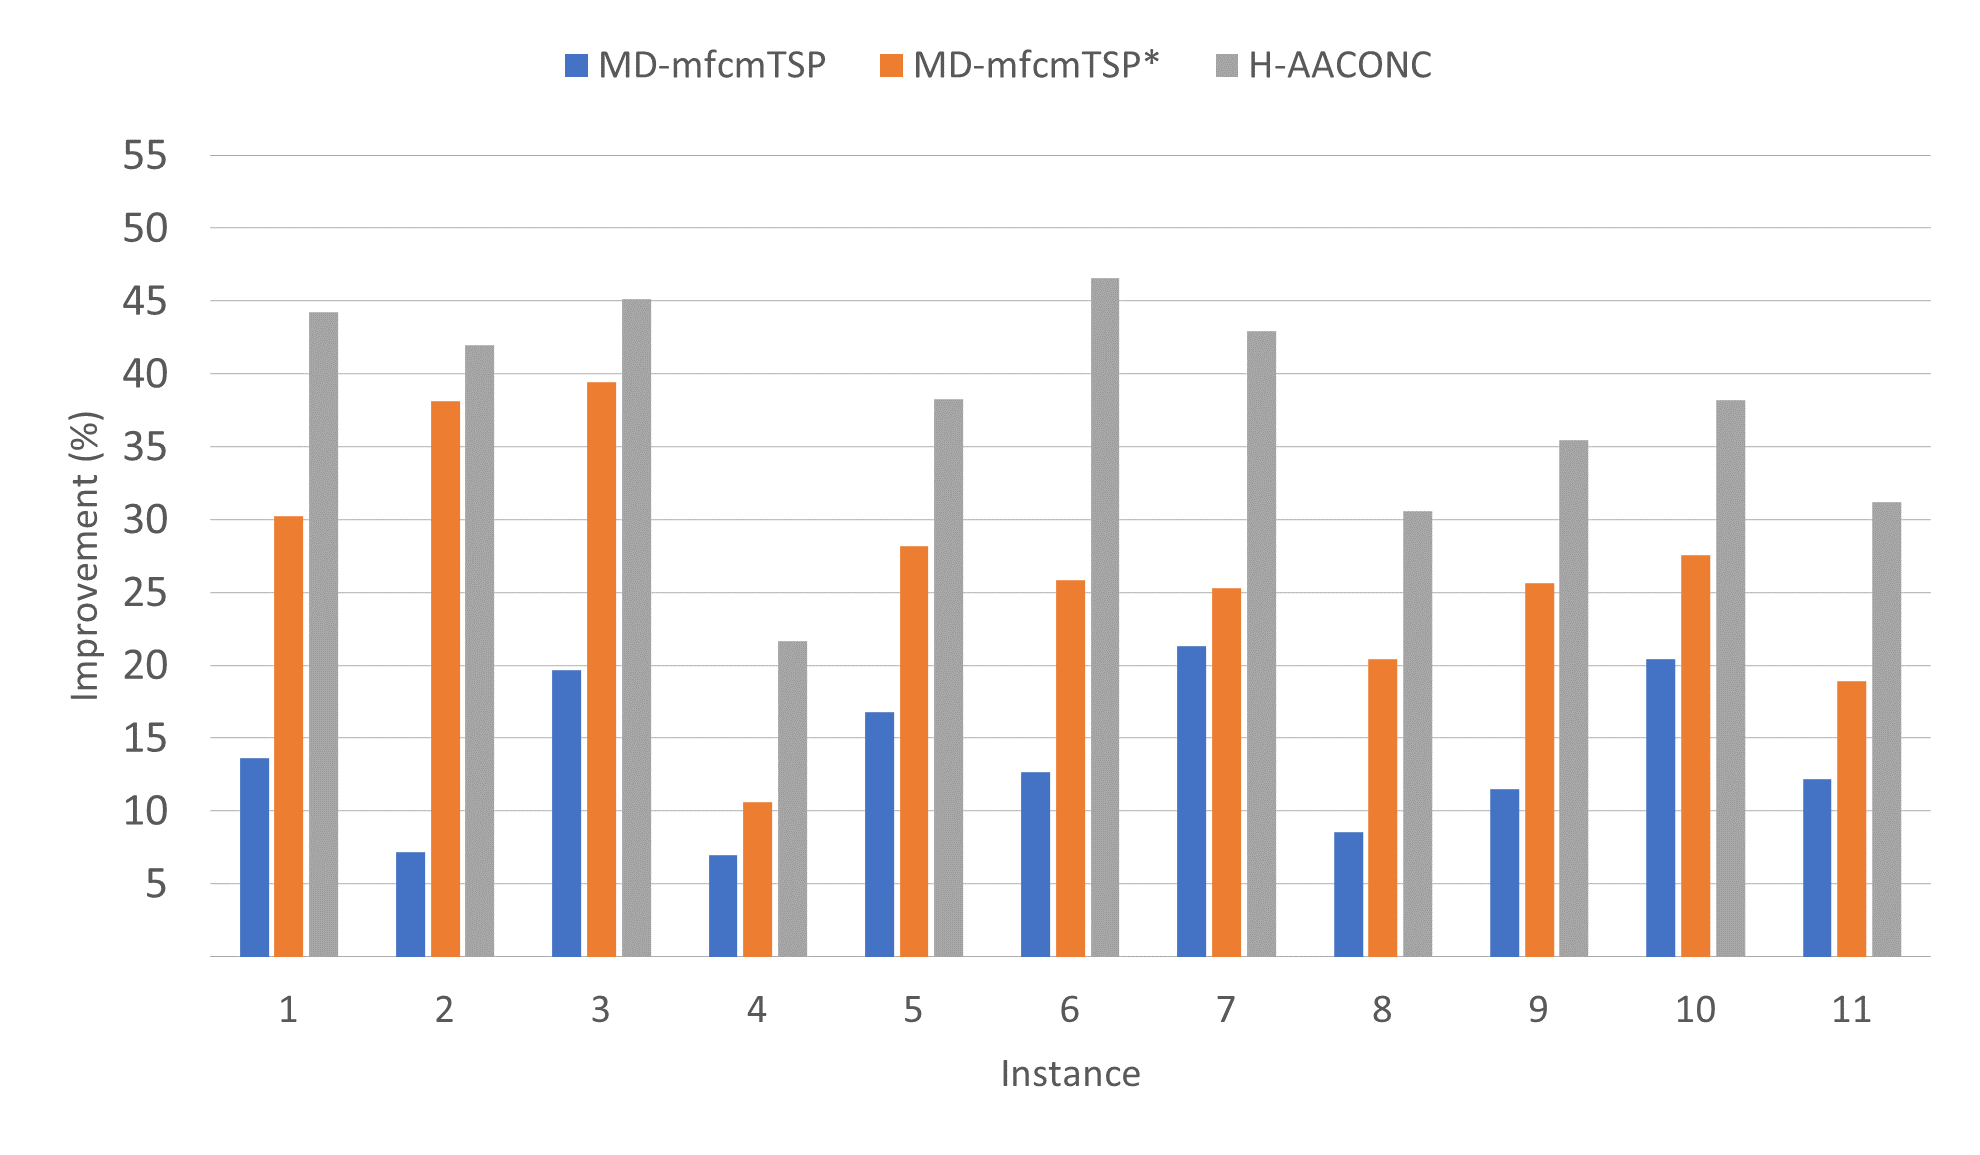
\includegraphics[scale=0.42]{small_15-15-15}\;
			\caption{$S_T=15$, $S_M=15$, $S_D=15$}
			\label{fig:15-15-15}
		\end{minipage}
		\begin{minipage}{0.33\textwidth}
			\centering
			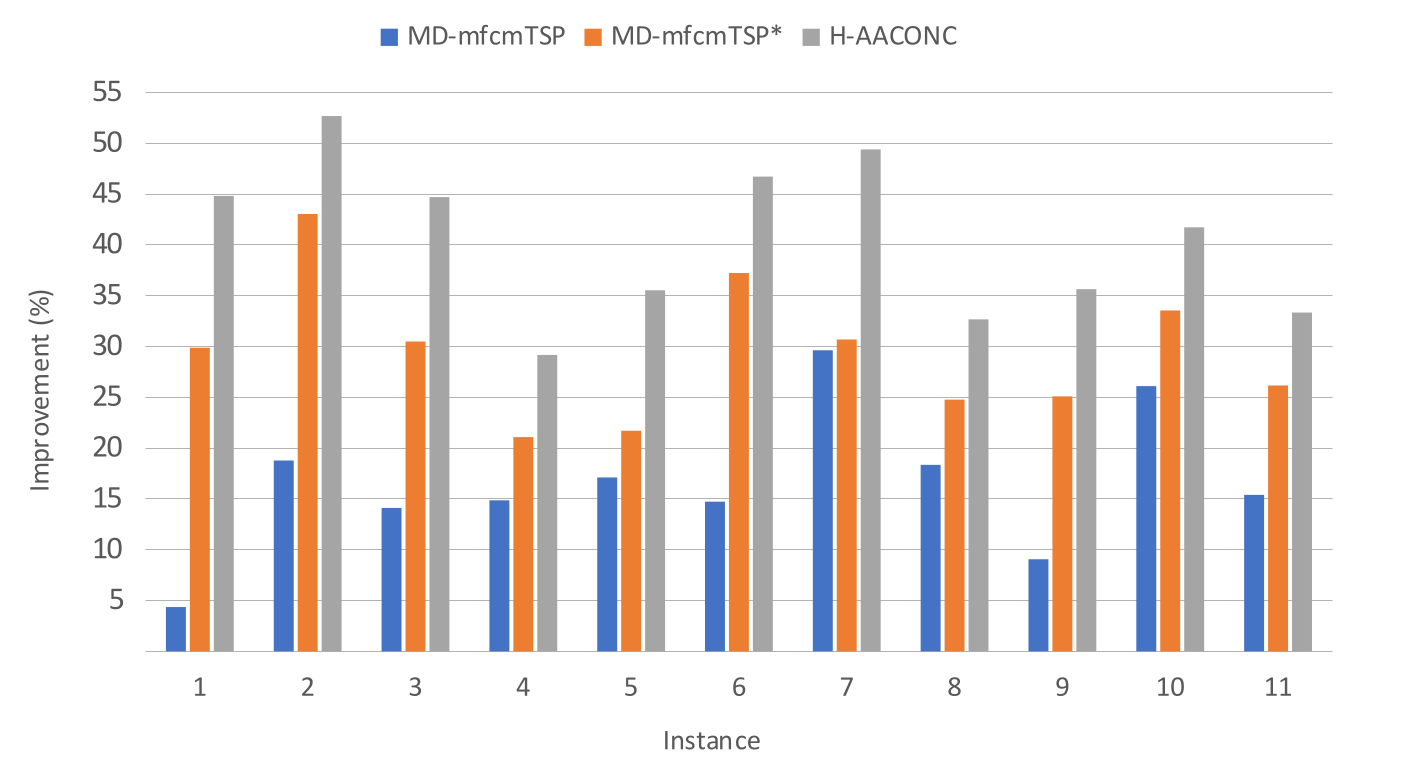
\includegraphics[scale=0.42]{small_15-20-20}\;
			\caption{$S_T=15$, $S_M=20$, $S_D=20$}
			\label{fig:15-20-20}
		\end{minipage}
		\begin{minipage}{0.33\textwidth}
			\centering
			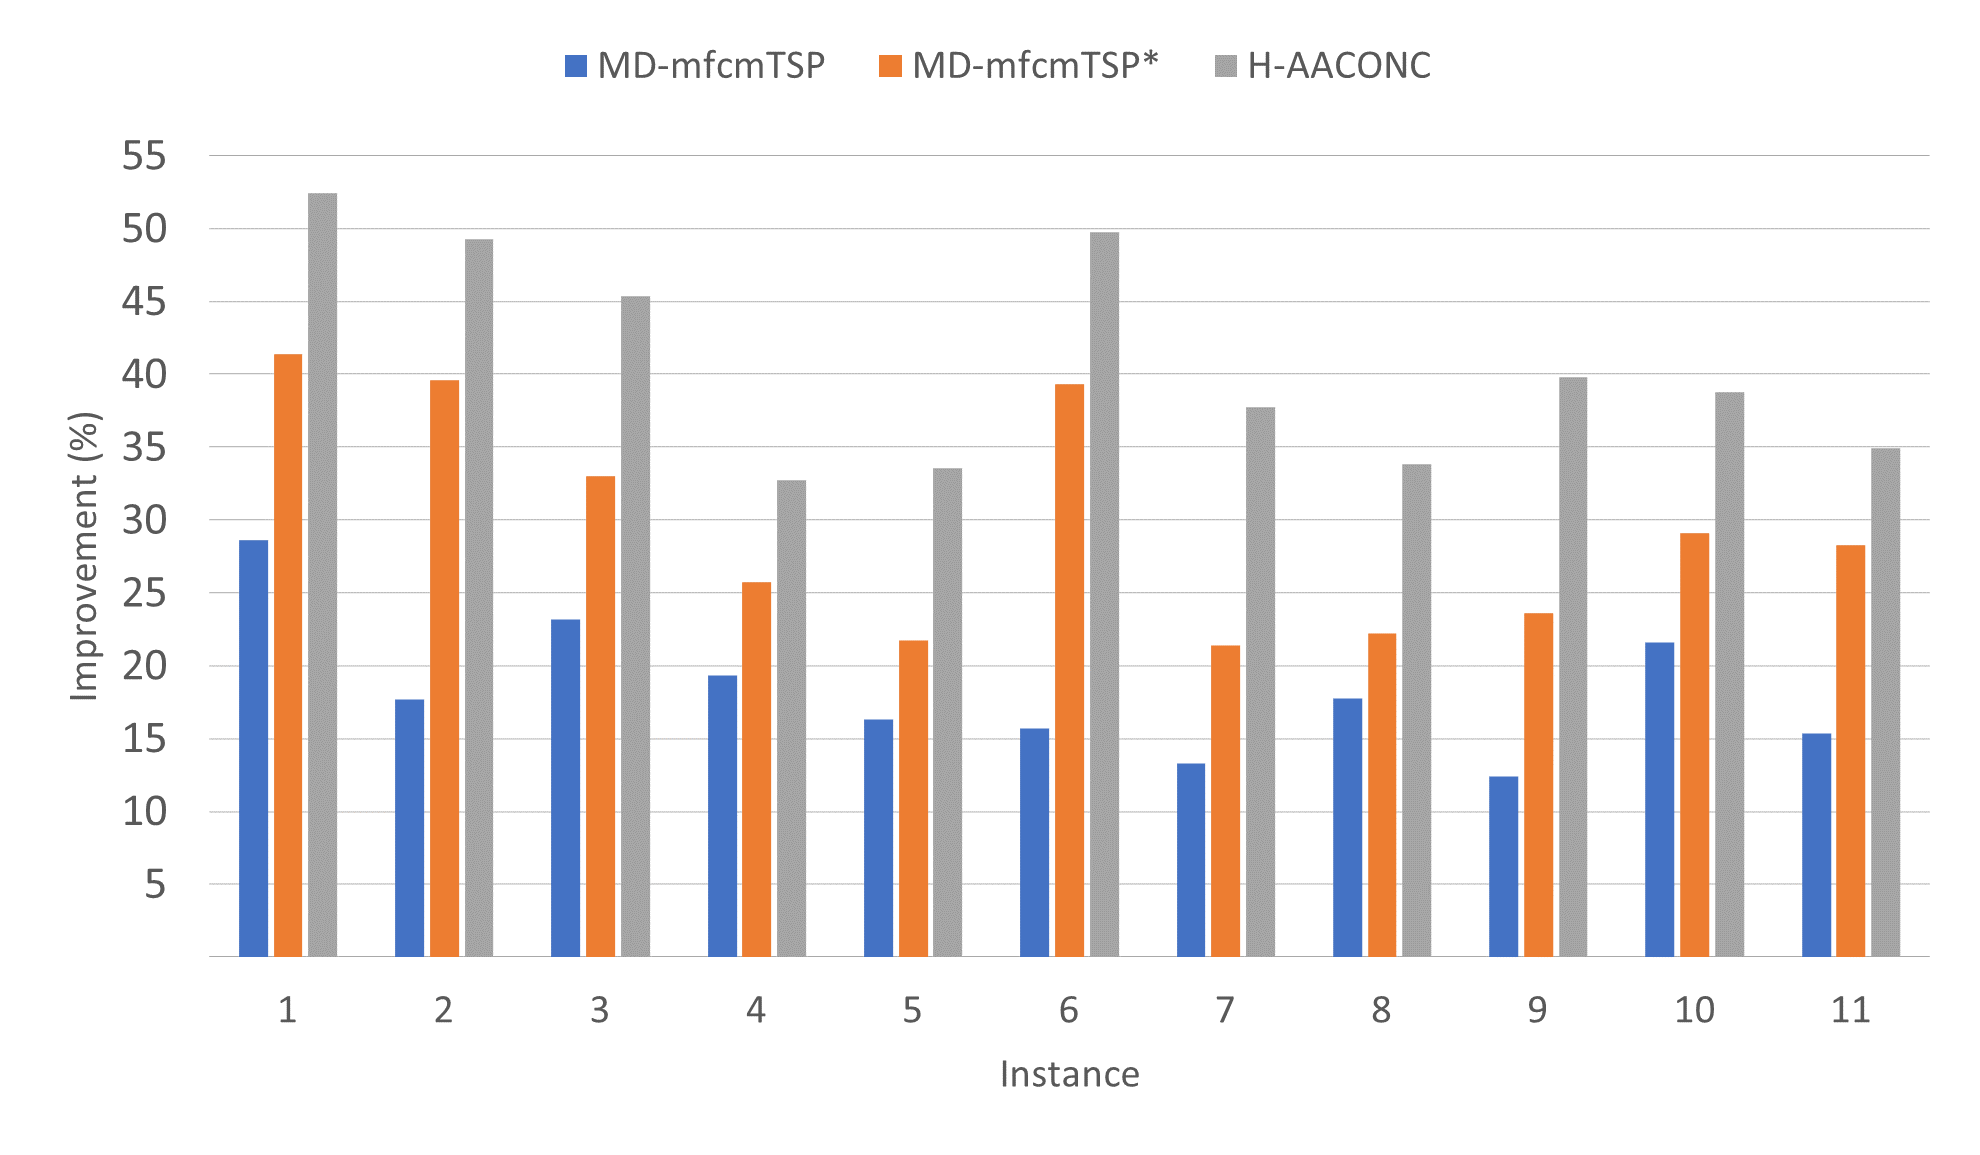
\includegraphics[scale=0.42]{small_15-20-30}\;
			\caption{$S_T=15$, $S_M=20$, $S_D=30$}
			\label{fig:15-20-30}
		\end{minipage}
	\end{figure}
	
	%Large instances
	\begin{figure}[h]
		\centering
		\begin{minipage}{0.33\textwidth}
			\centering
			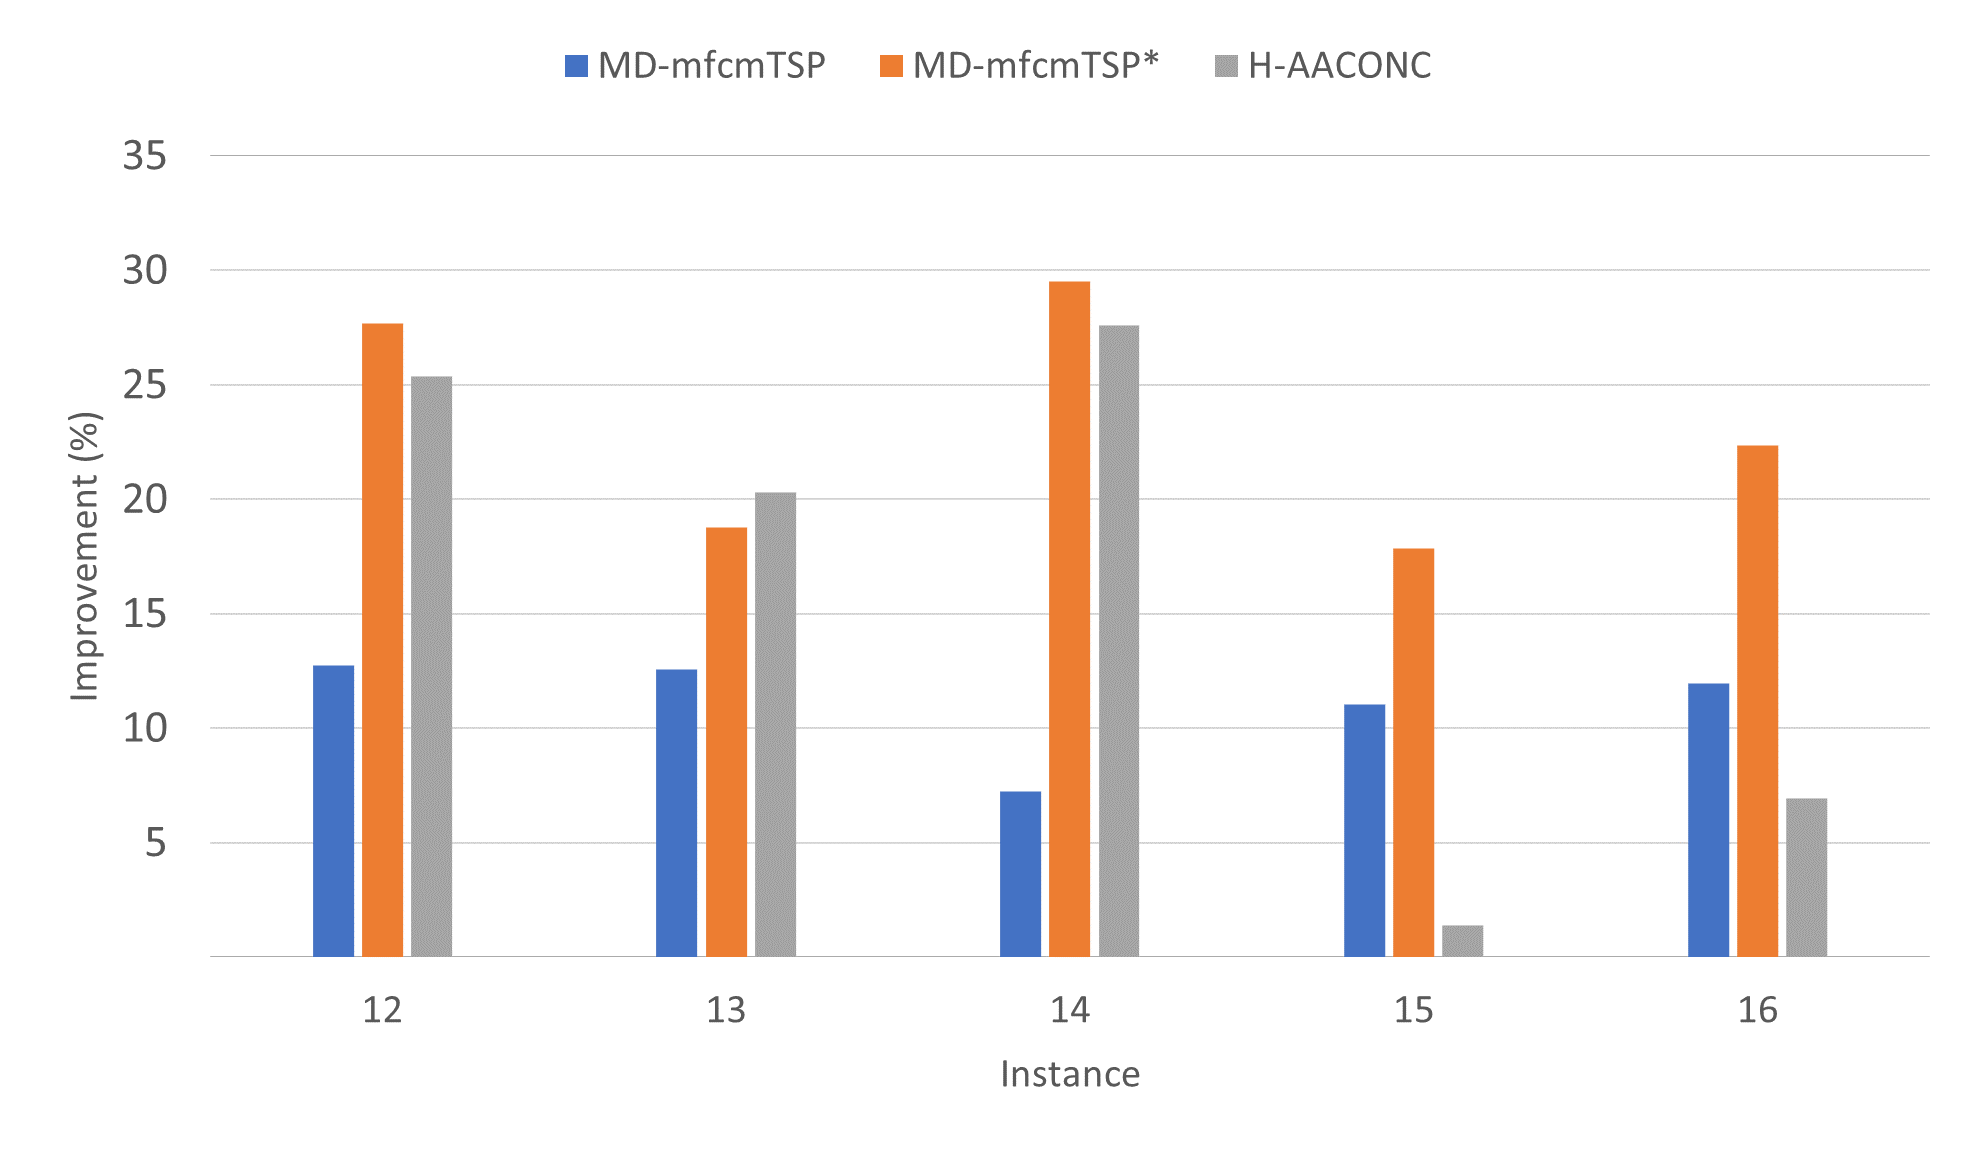
\includegraphics[scale=0.42]{large_15-15-15}\;
			\caption{$S_T=15$, $S_M=15$, $S_D=15$}
			\label{fig:large_15-15-15}
		\end{minipage}
		\begin{minipage}{0.33\textwidth}
			\centering
			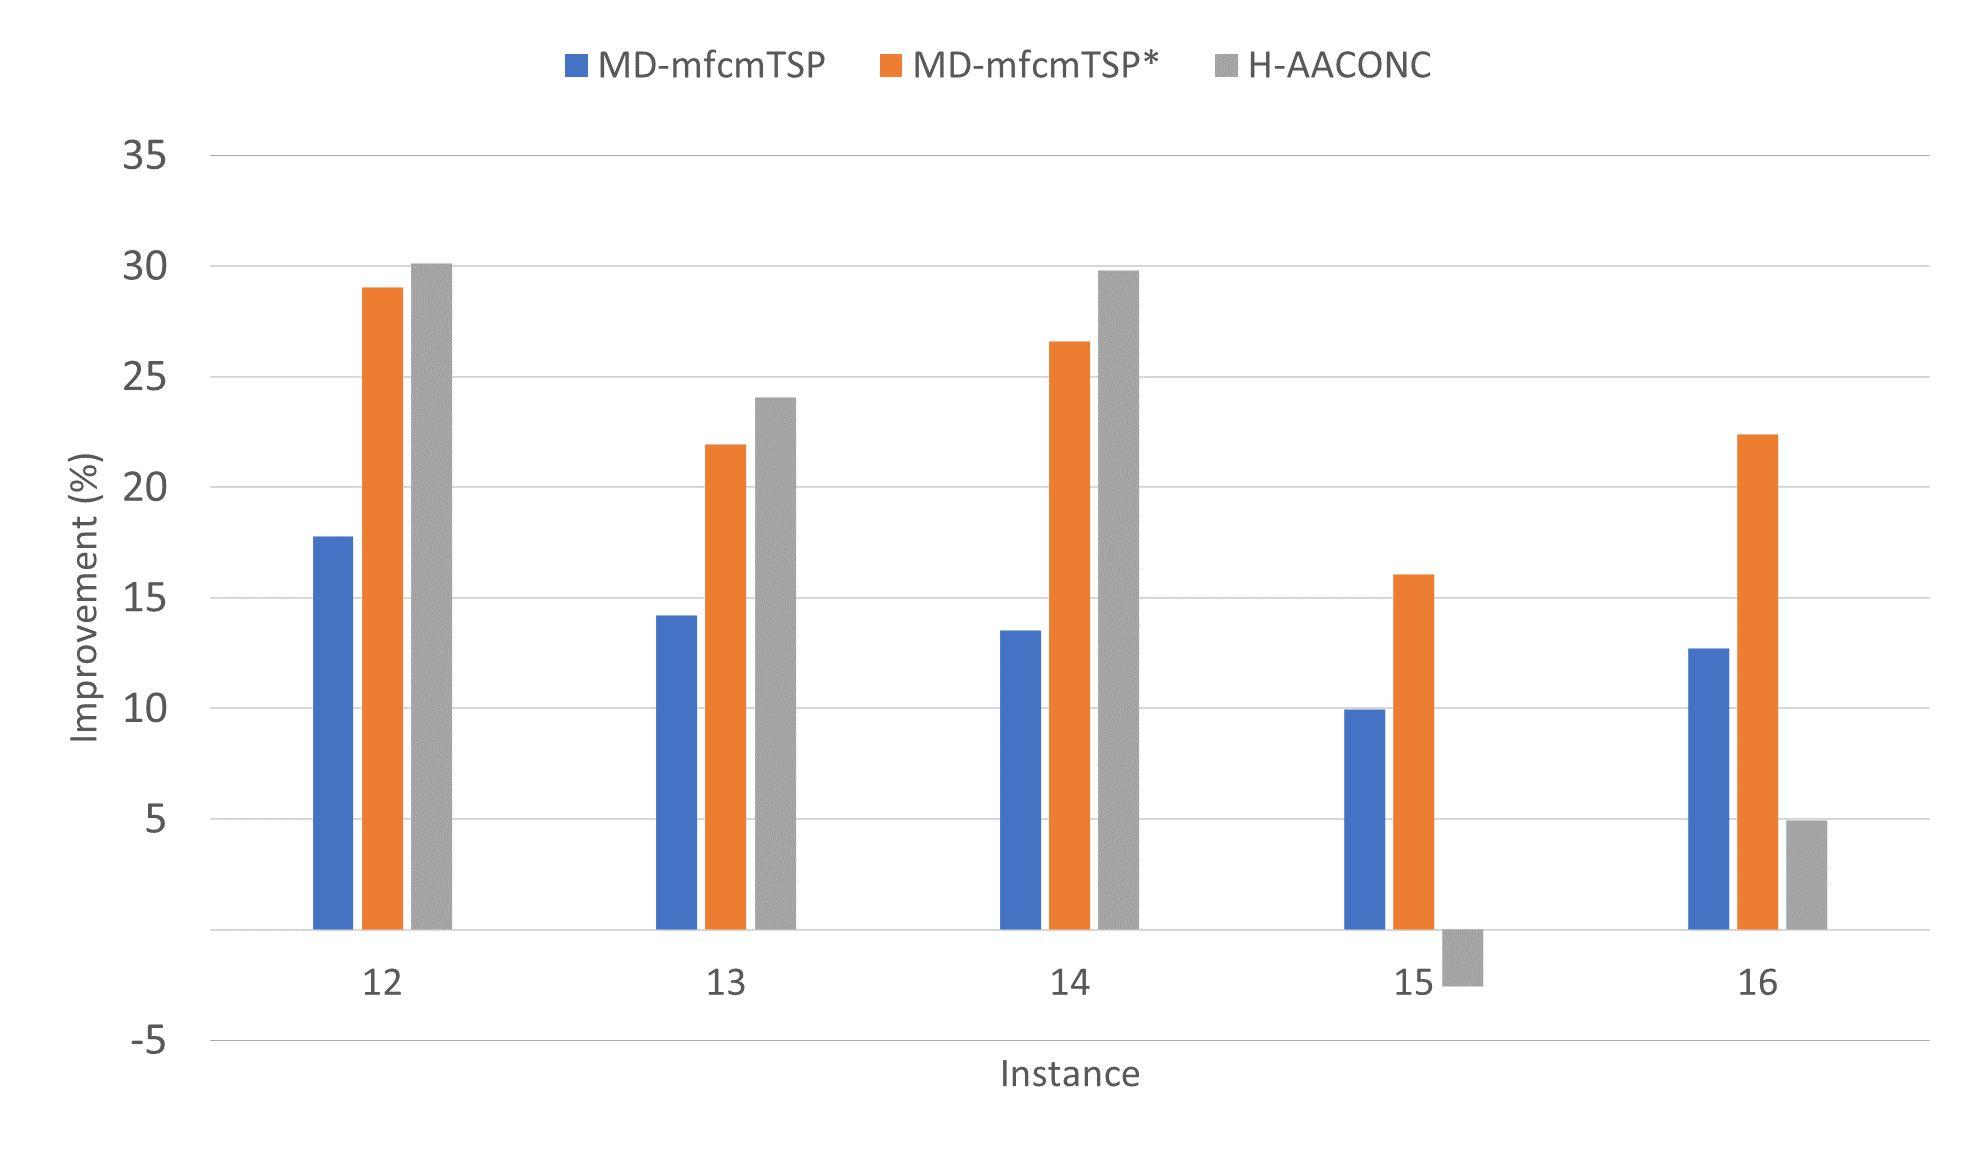
\includegraphics[scale=0.42]{large_15-20-20}\;
			\caption{$S_T=15$, $S_M=20$, $S_D=20$}
			\label{fig:large_15-20-20}
		\end{minipage}
		\begin{minipage}{0.33\textwidth}
			\centering
			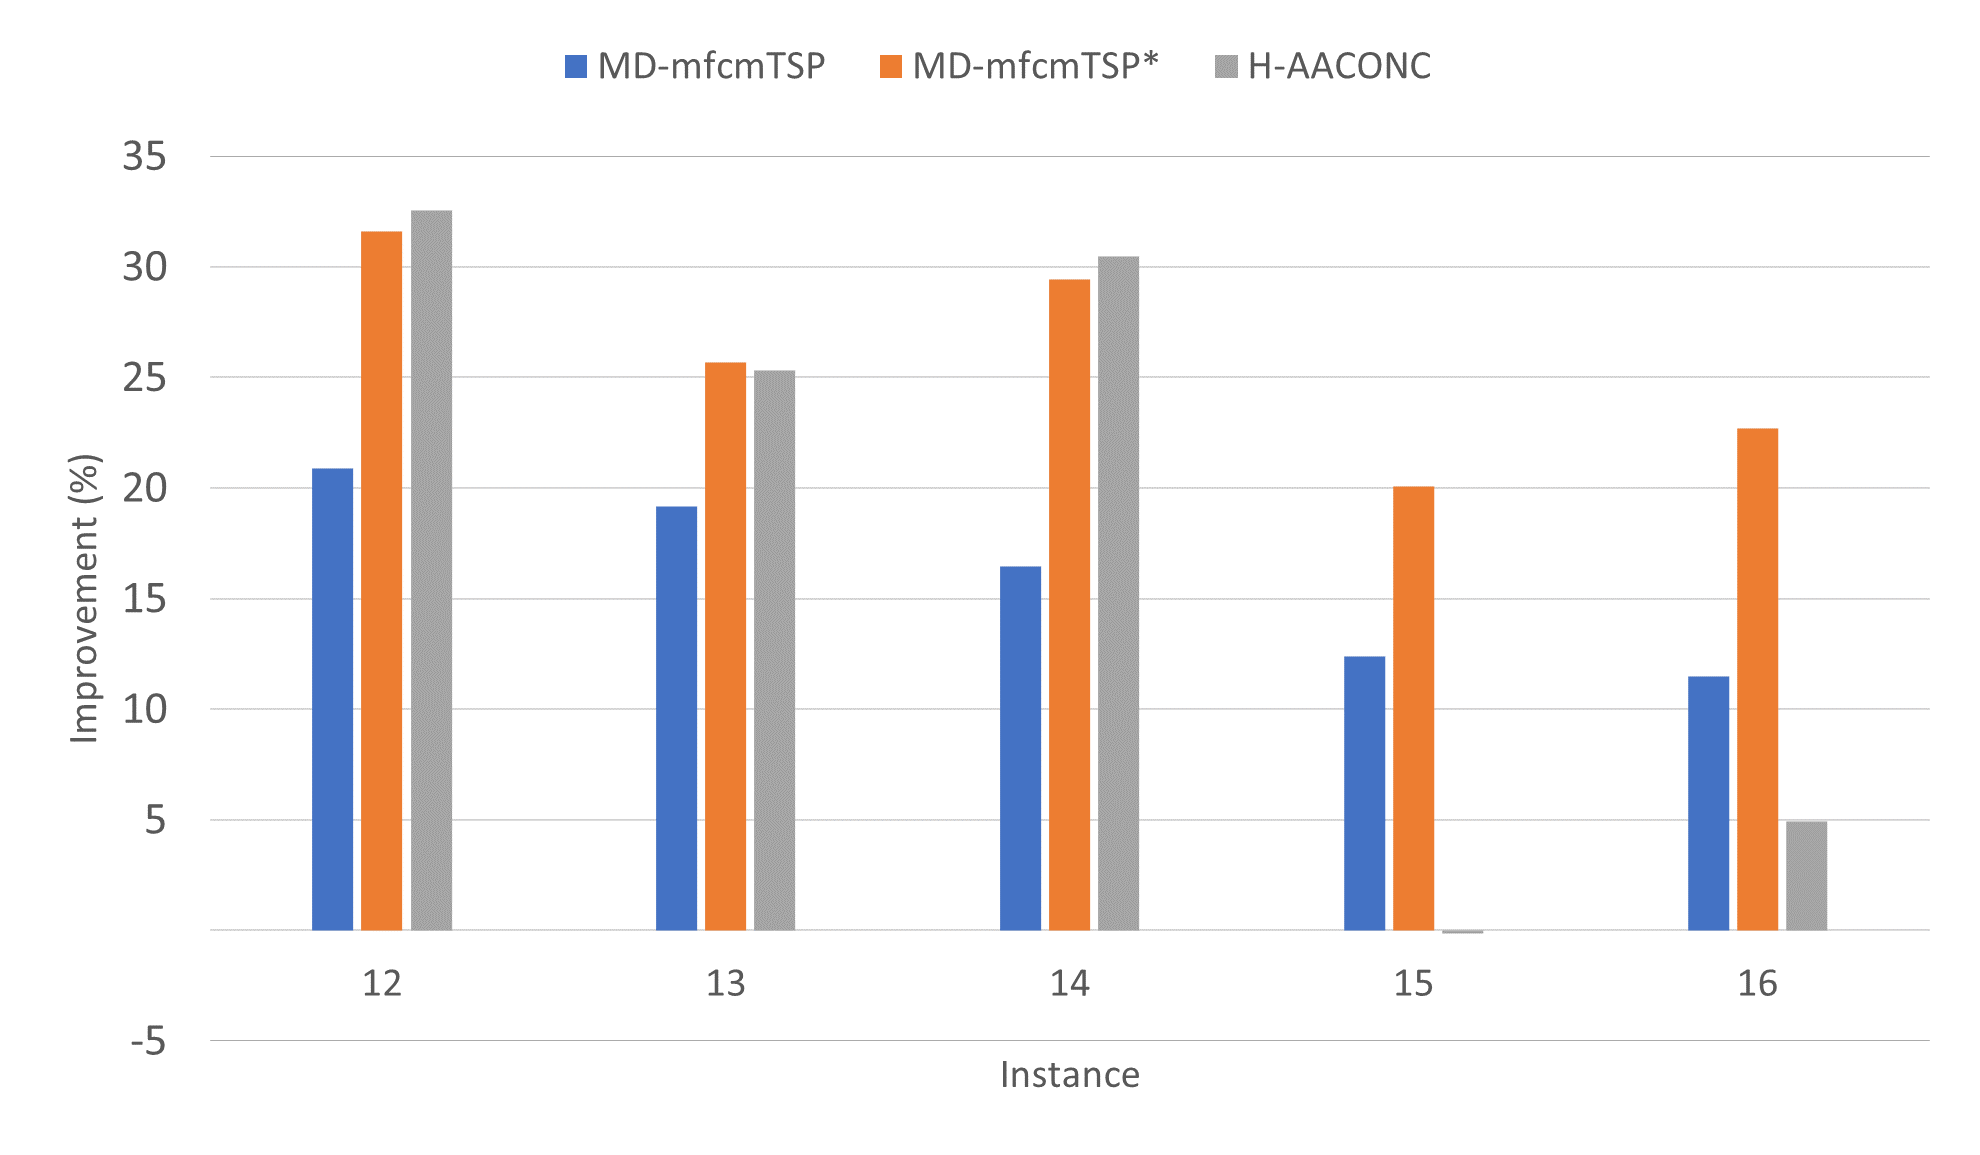
\includegraphics[scale=0.42]{large_15-20-30}\;
			\caption{$S_T=15$, $S_M=20$, $S_D=30$}
			\label{fig:large_15-20-30}
		\end{minipage}
	\end{figure}
	
	%Motorbike experiments 07
	\begin{figure}[h]
		\centering
		\begin{minipage}{0.33\textwidth}
			\centering
			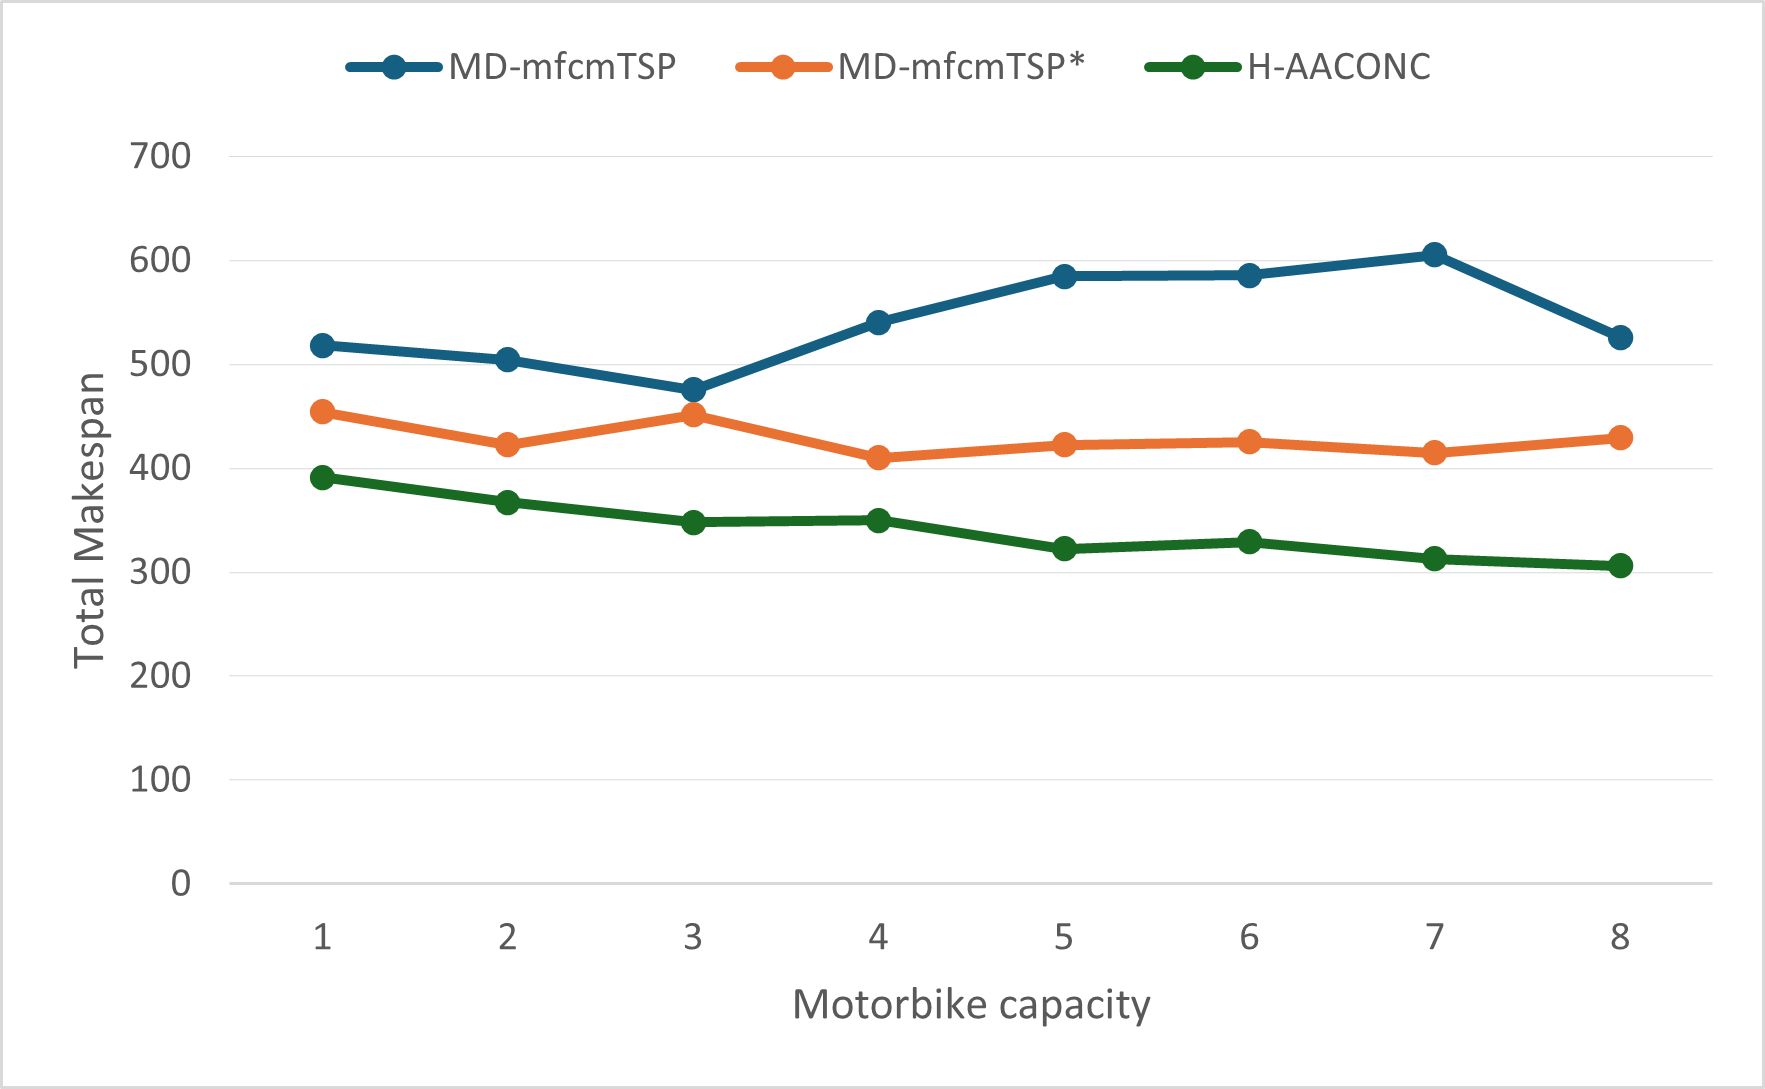
\includegraphics[scale=0.42]{p07_NM1}\;
			\caption{Instance 7 - $N_M=1$}
			\label{fig:p07_NM1}
		\end{minipage}
		\begin{minipage}{0.33\textwidth}
			\centering
			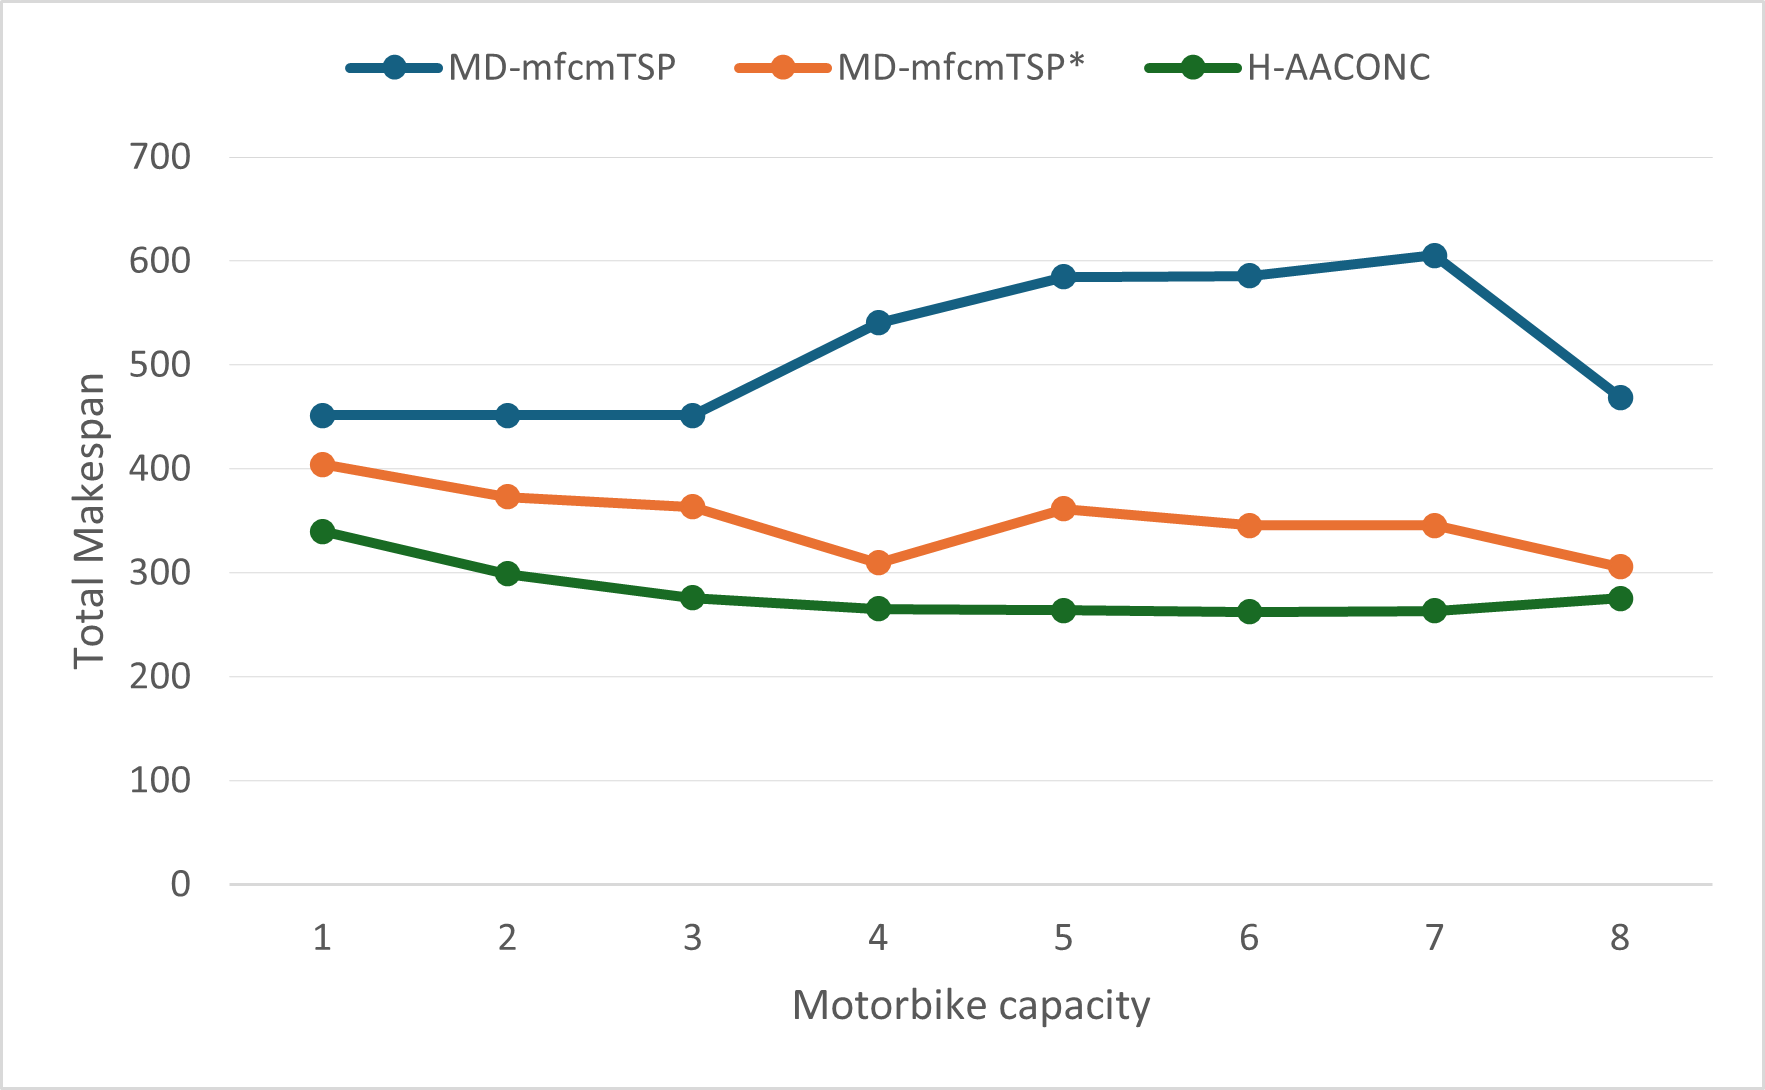
\includegraphics[scale=0.42]{p07_NM2}\;
			\caption{Instance 7 - $N_M=2$}
			\label{fig:p07_NM2}
		\end{minipage}
		\begin{minipage}{0.33\textwidth}
			\centering
			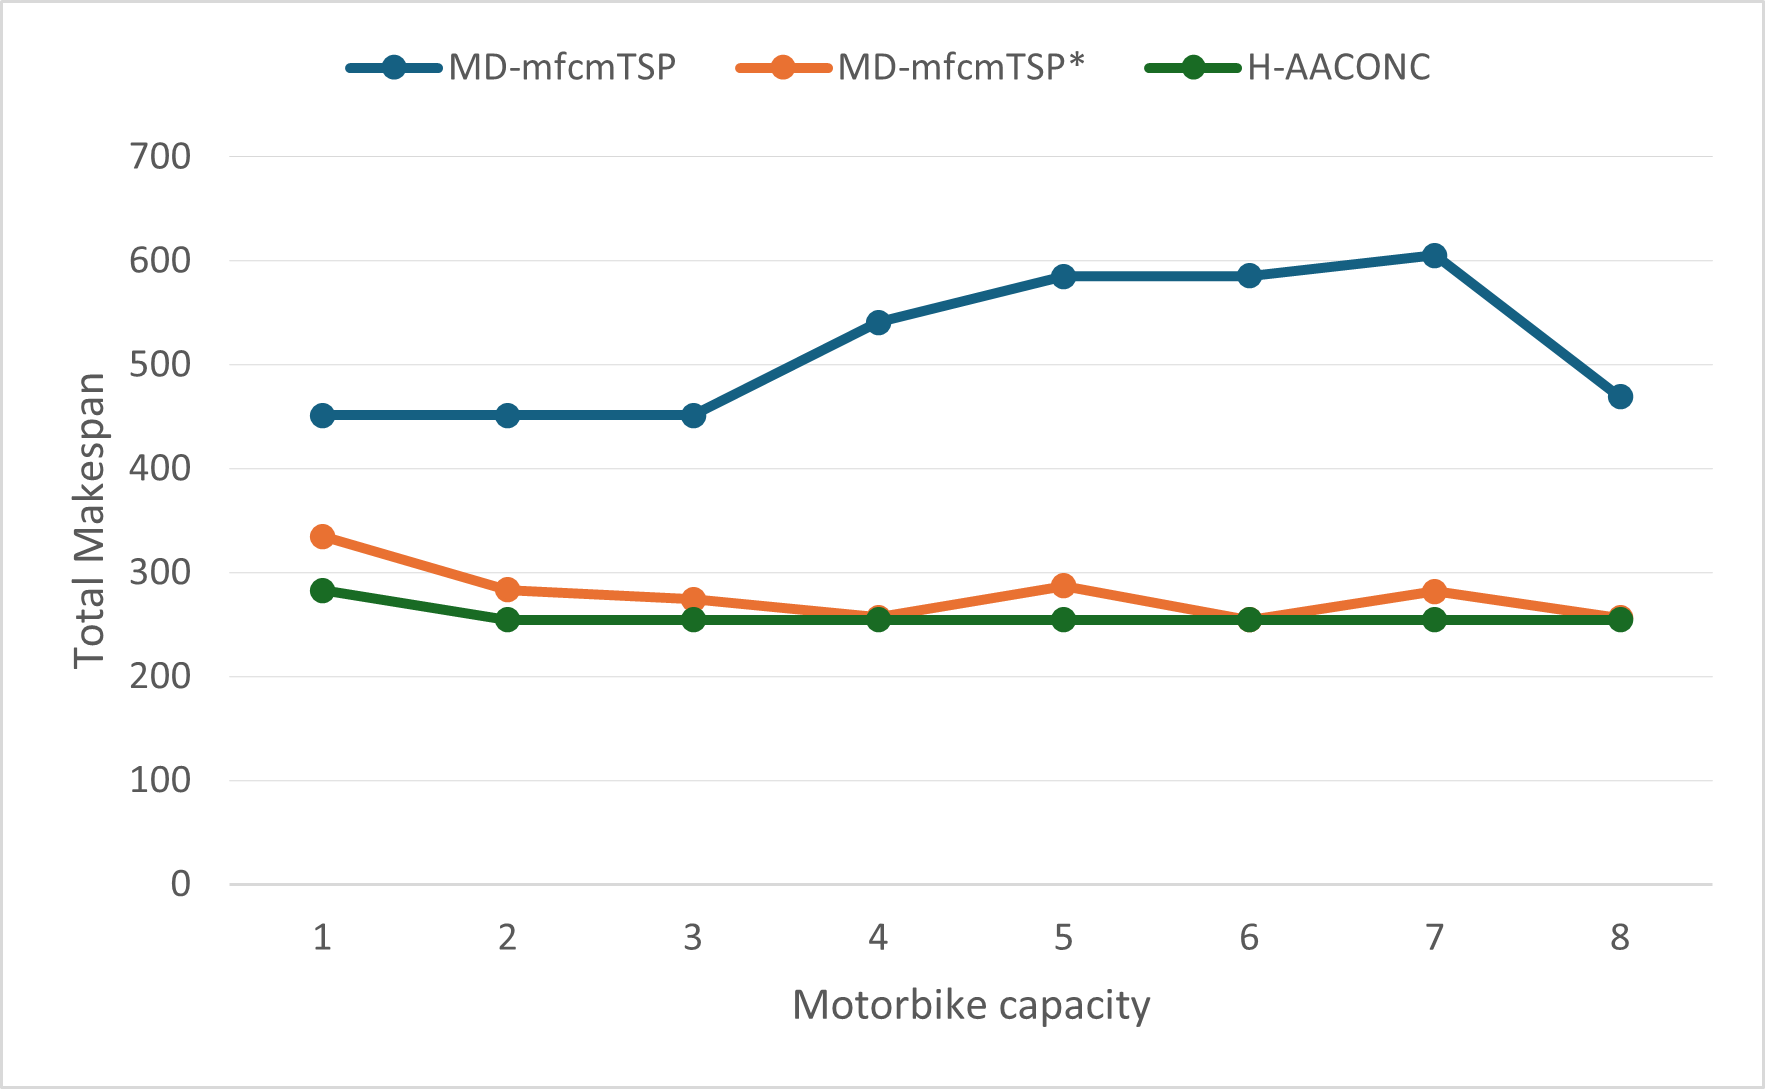
\includegraphics[scale=0.42]{p07_NM4}\;
			\caption{Instance 7 - $N_M=4$}
			\label{fig:p07_NM4}
		\end{minipage}
	\end{figure}
	
	%Motorbike experiments 11
	\begin{figure}[h]
		\centering
		\begin{minipage}{0.33\textwidth}
			\centering
			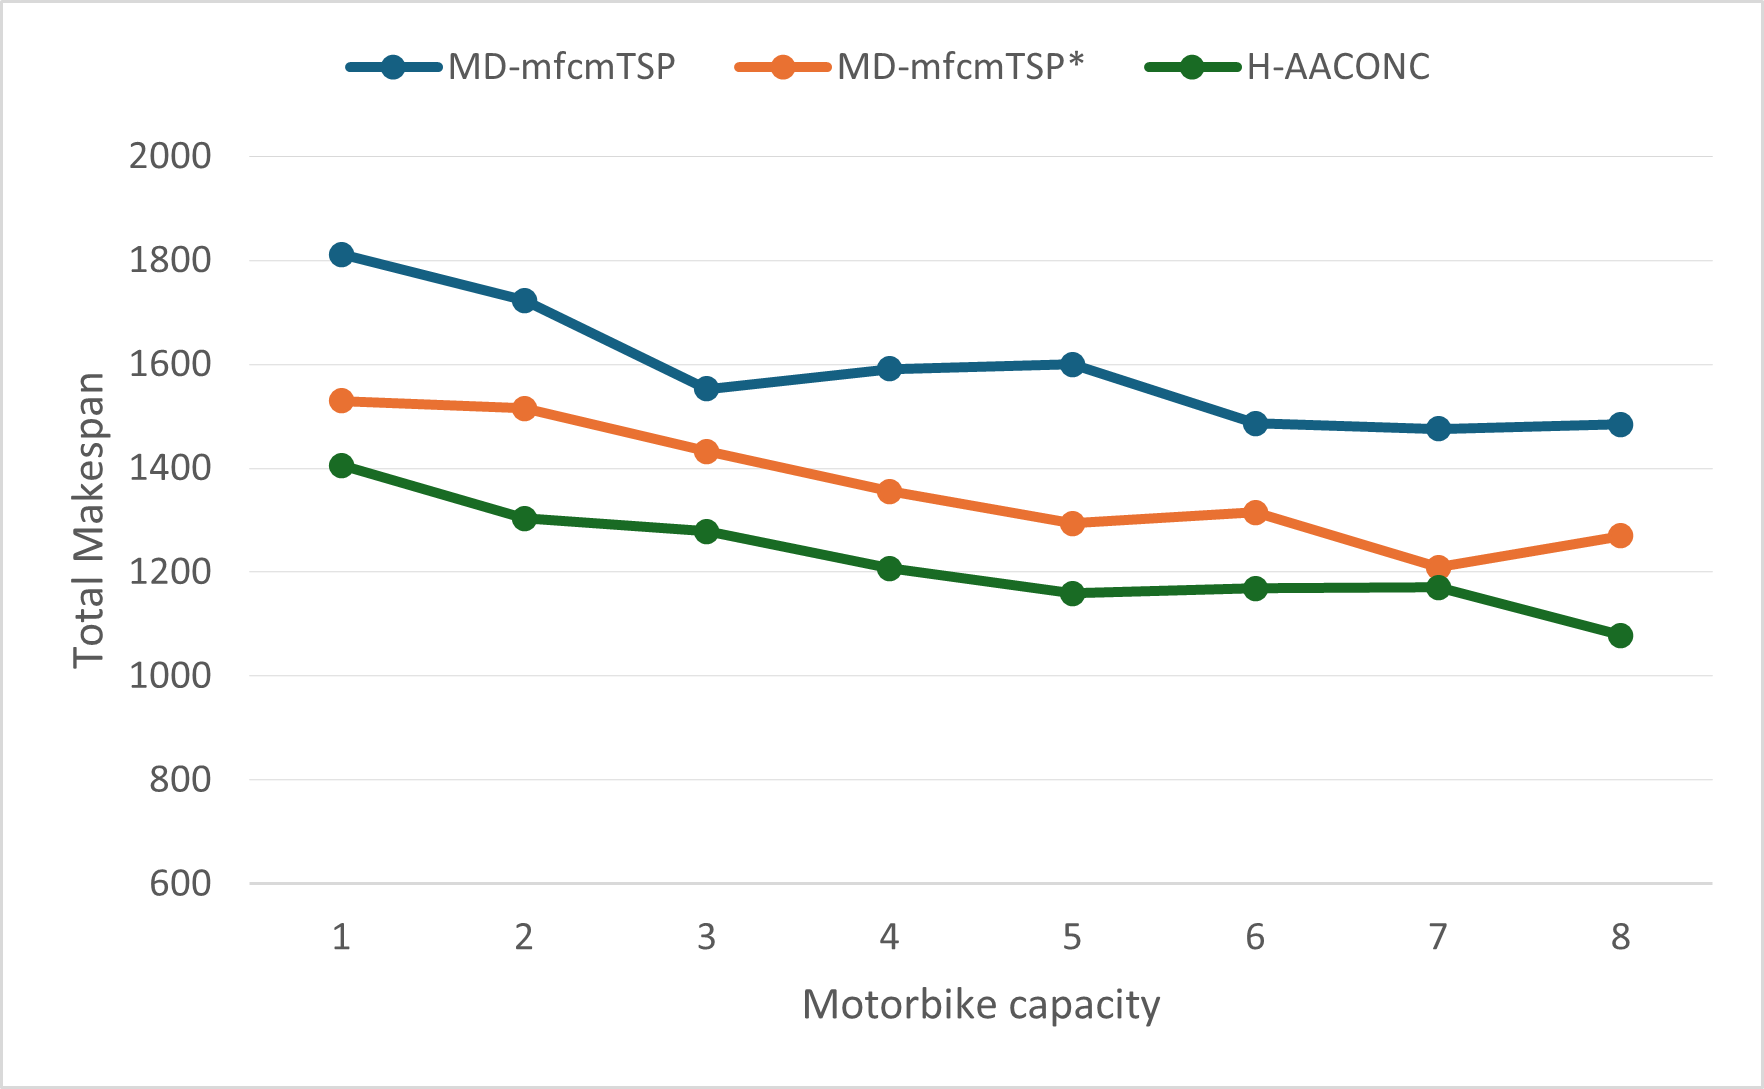
\includegraphics[scale=0.42]{p11_NM1}\;
			\caption{Instance 11 - $N_M=1$}
			\label{fig:p11_NM1}
		\end{minipage}
		\begin{minipage}{0.33\textwidth}
			\centering
			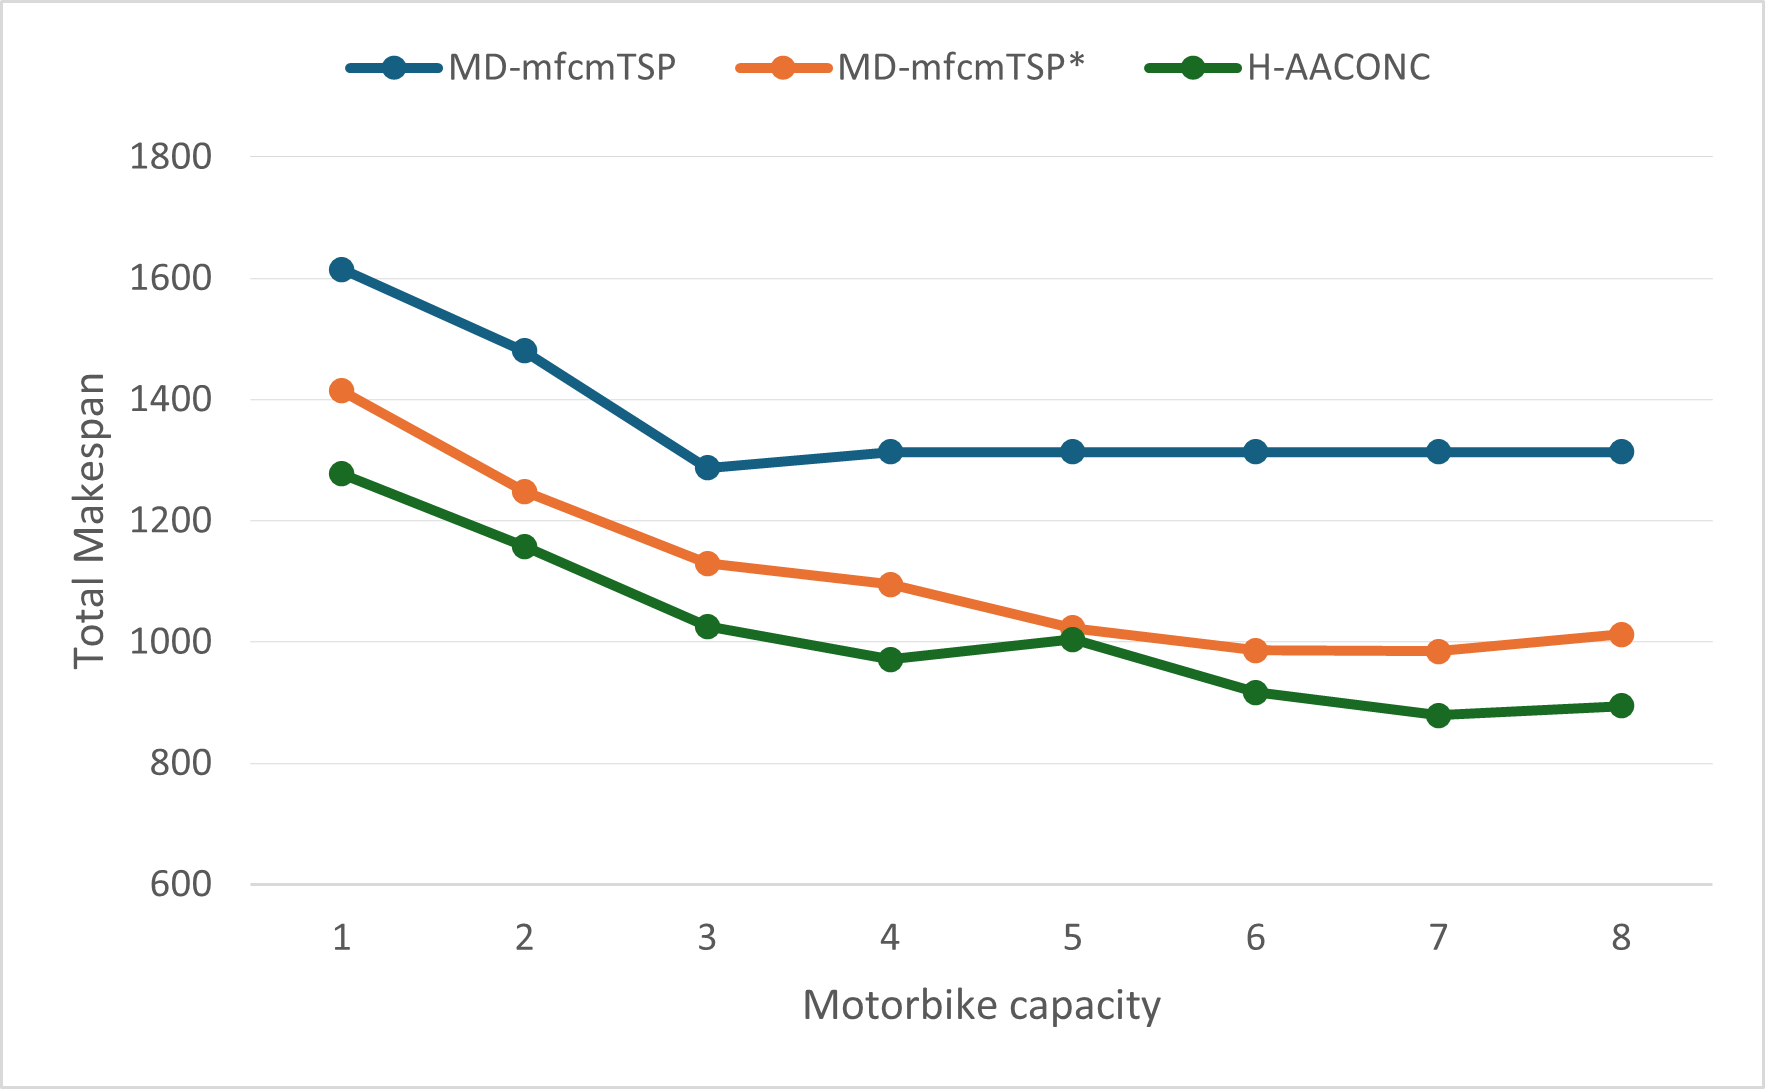
\includegraphics[scale=0.42]{p11_NM2}\;
			\caption{Instance 11 - $N_M=2$}
			\label{fig:p11_NM2}
		\end{minipage}
		\begin{minipage}{0.33\textwidth}
			\centering
			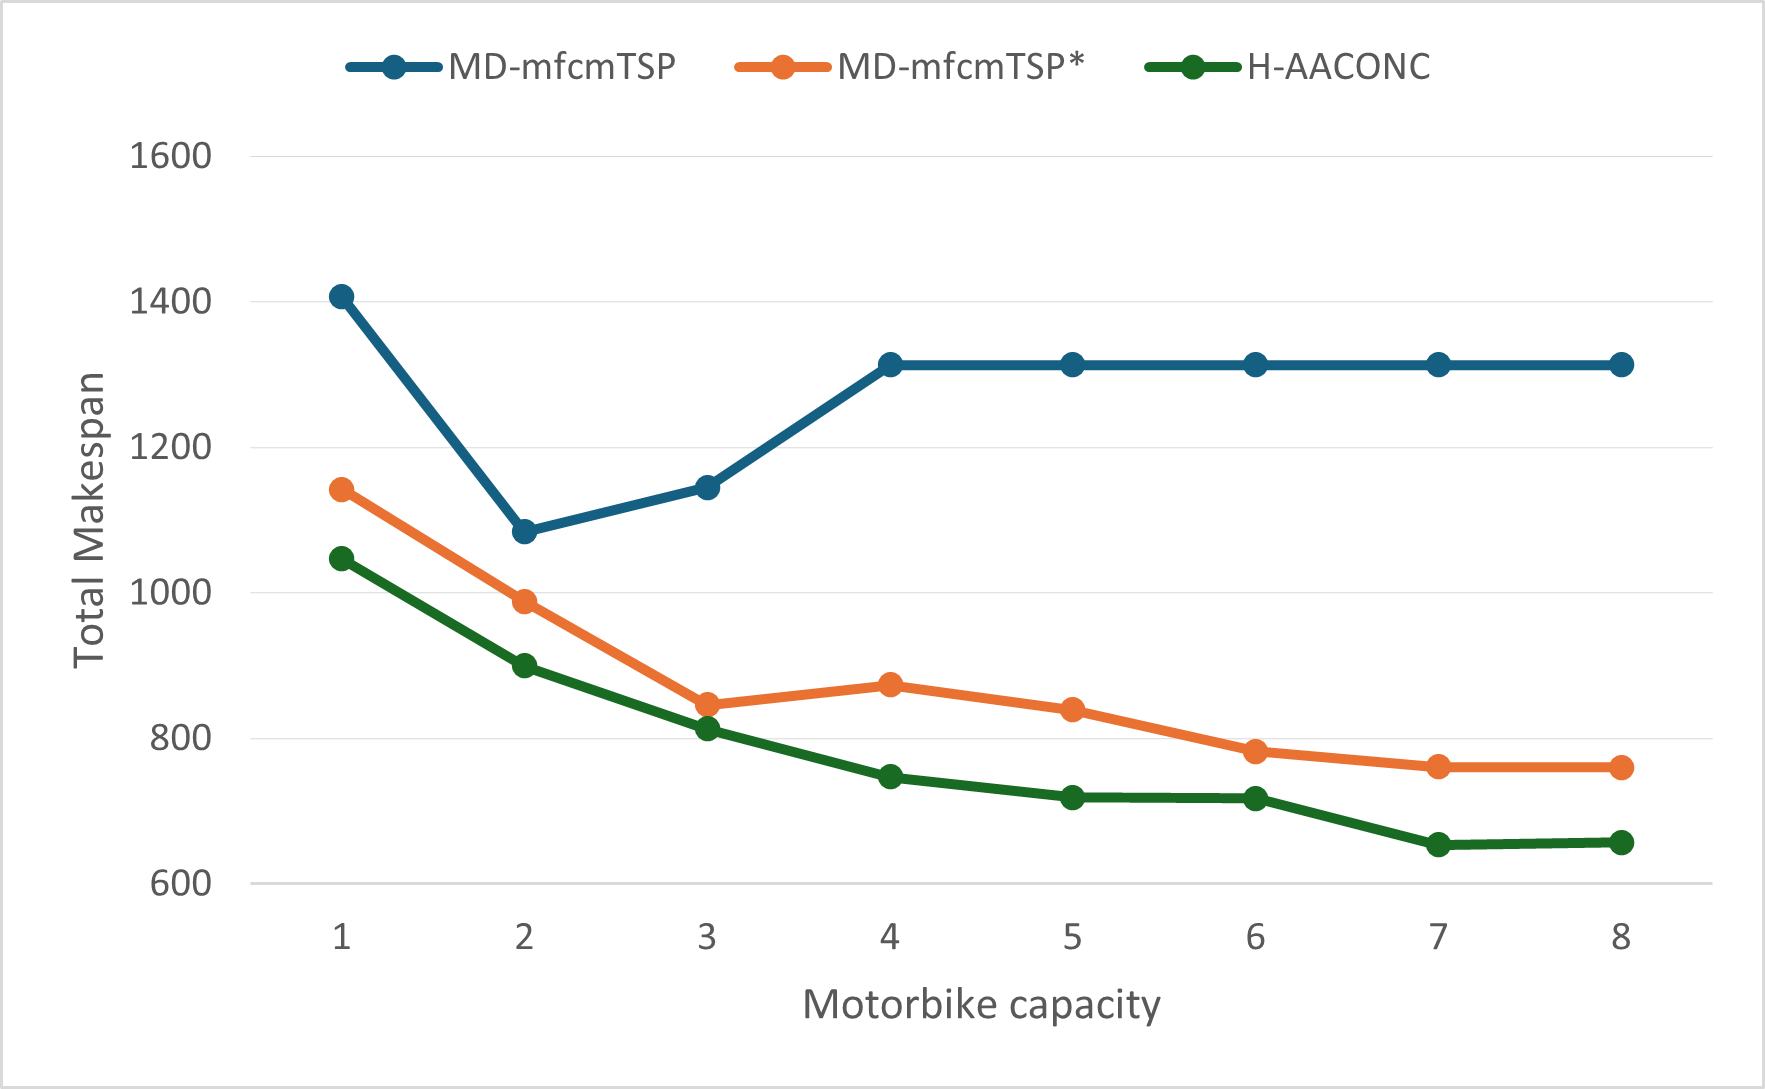
\includegraphics[scale=0.42]{p11_NM4}\;
			\caption{Instance 11 - $N_M=4$}
			\label{fig:p11_NM4}
		\end{minipage}
	\end{figure}
	
	%Drone experiments 07
	\begin{figure}[h]
		\centering
		\begin{minipage}{0.33\textwidth}
			\centering
			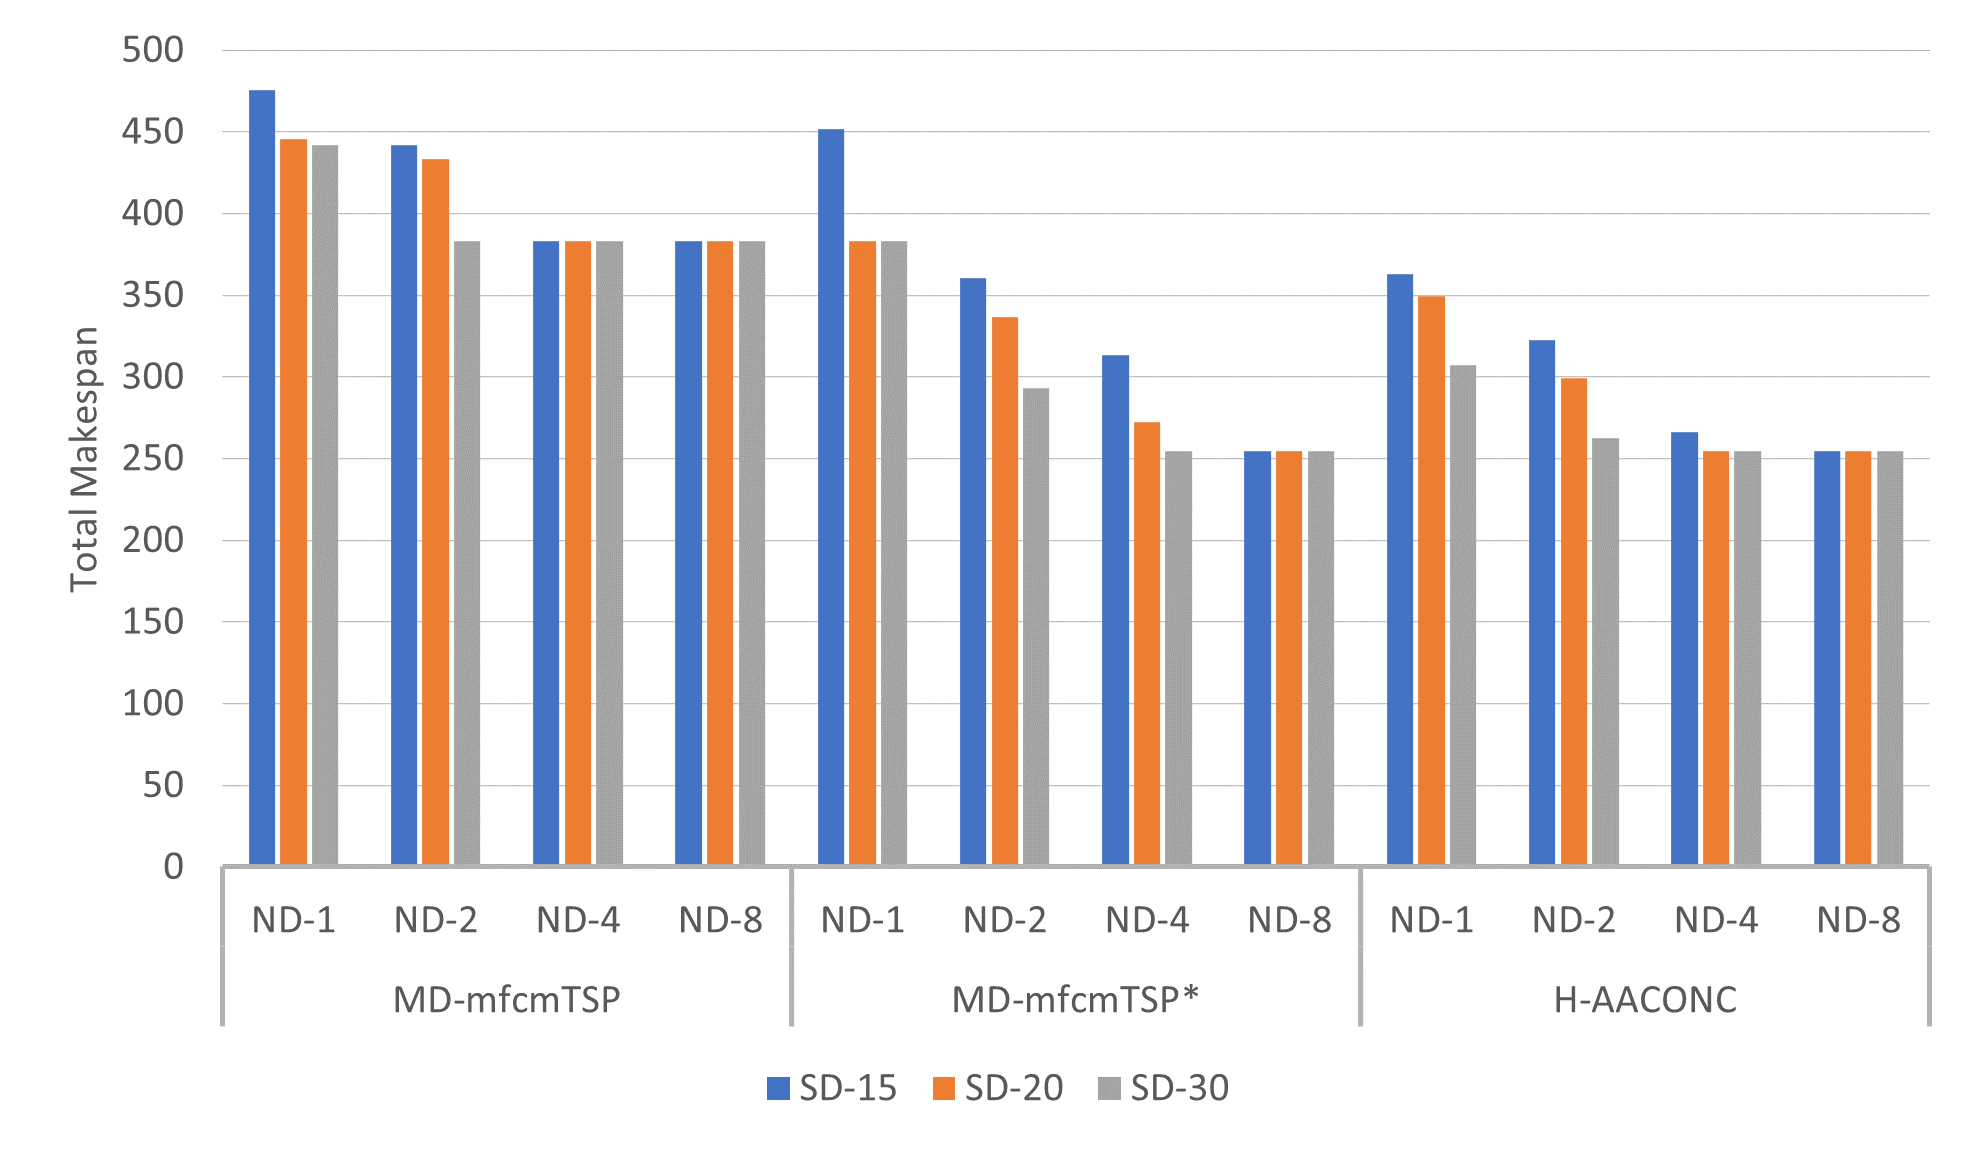
\includegraphics[scale=0.42]{p07_drones}\;
			\caption{Instance 7}
			\label{fig:p07_drones}
		\end{minipage}
		\begin{minipage}{0.33\textwidth}
			\centering
			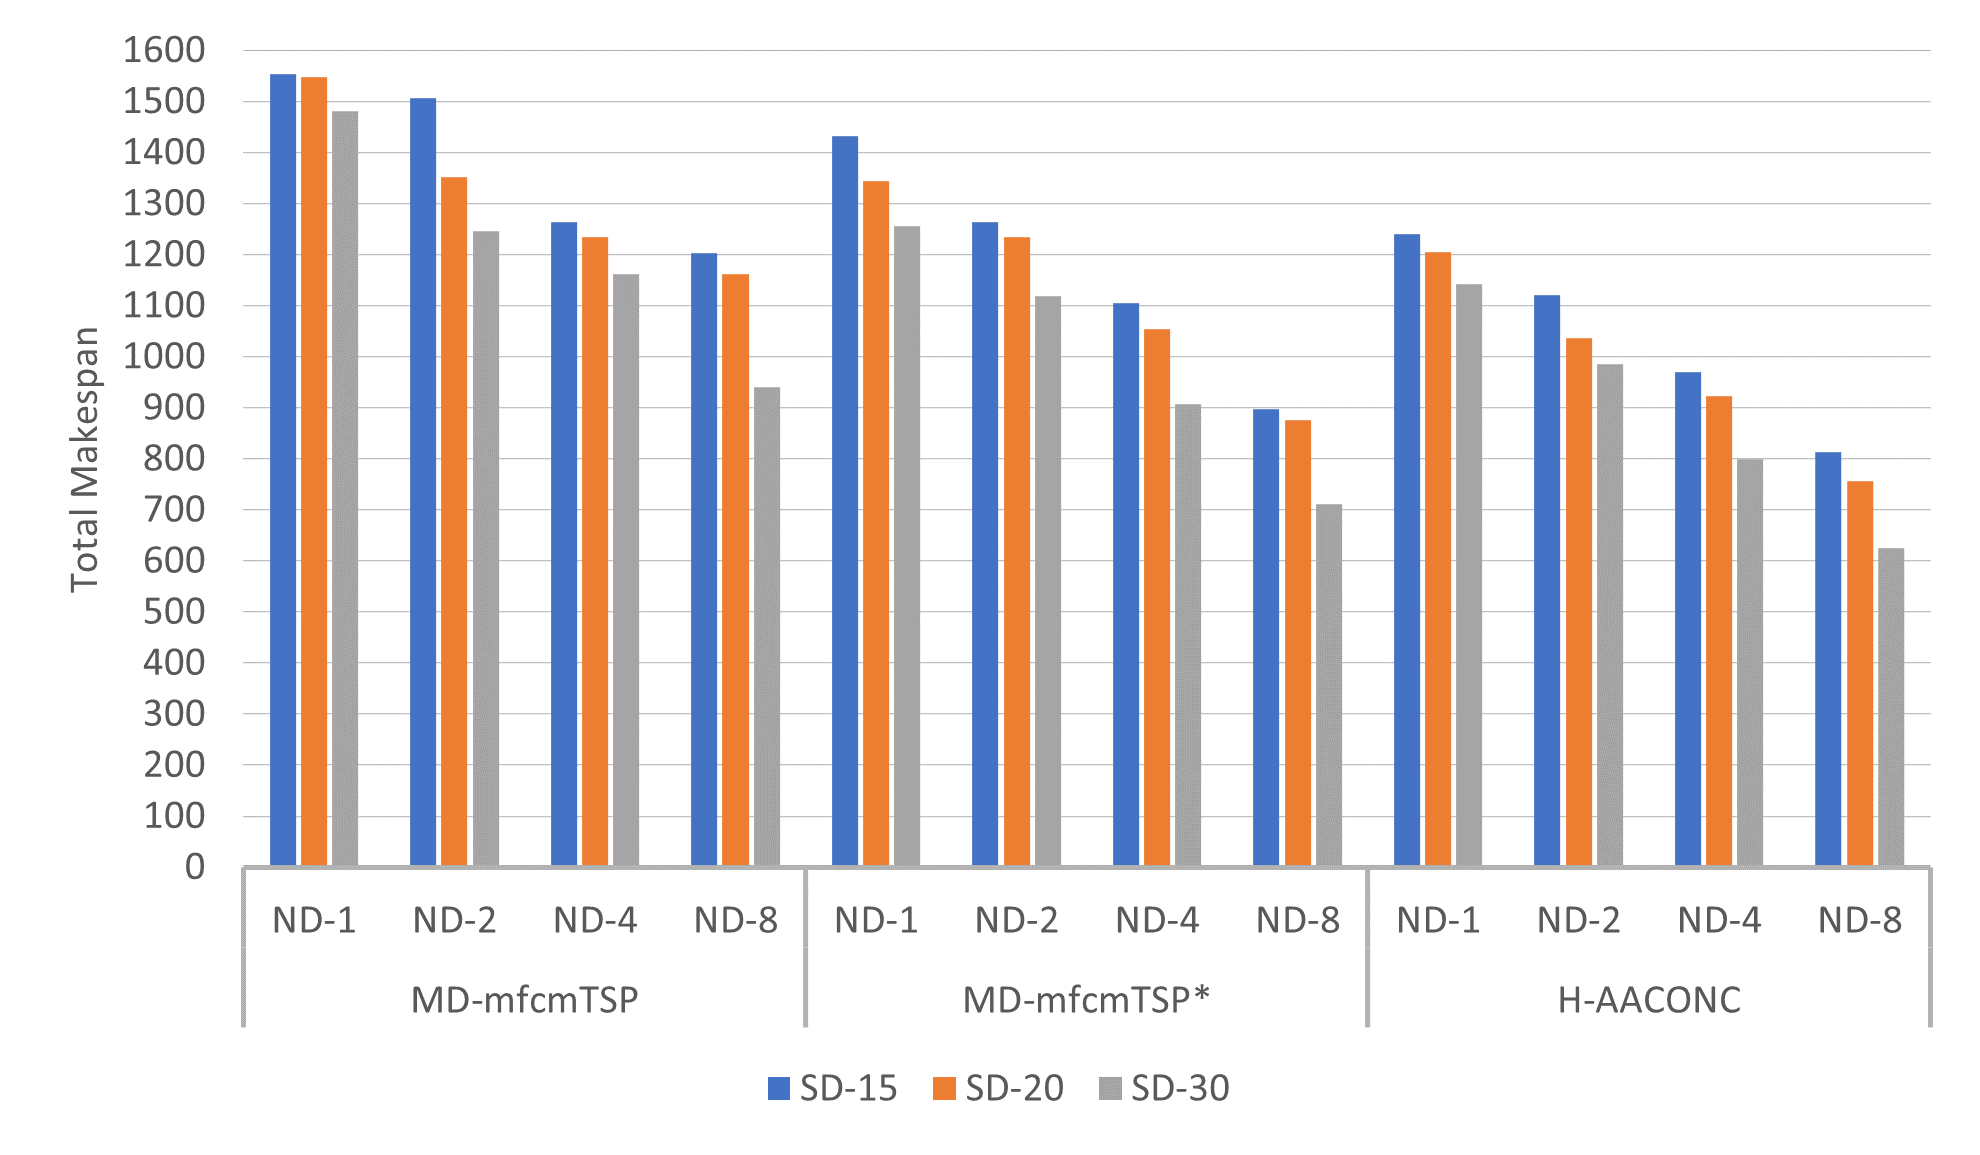
\includegraphics[scale=0.42]{p11_drones}\;
			\caption{Instance 11}
			\label{fig:p11_drones}
		\end{minipage}
		\begin{minipage}{0.33\textwidth}
			\centering
			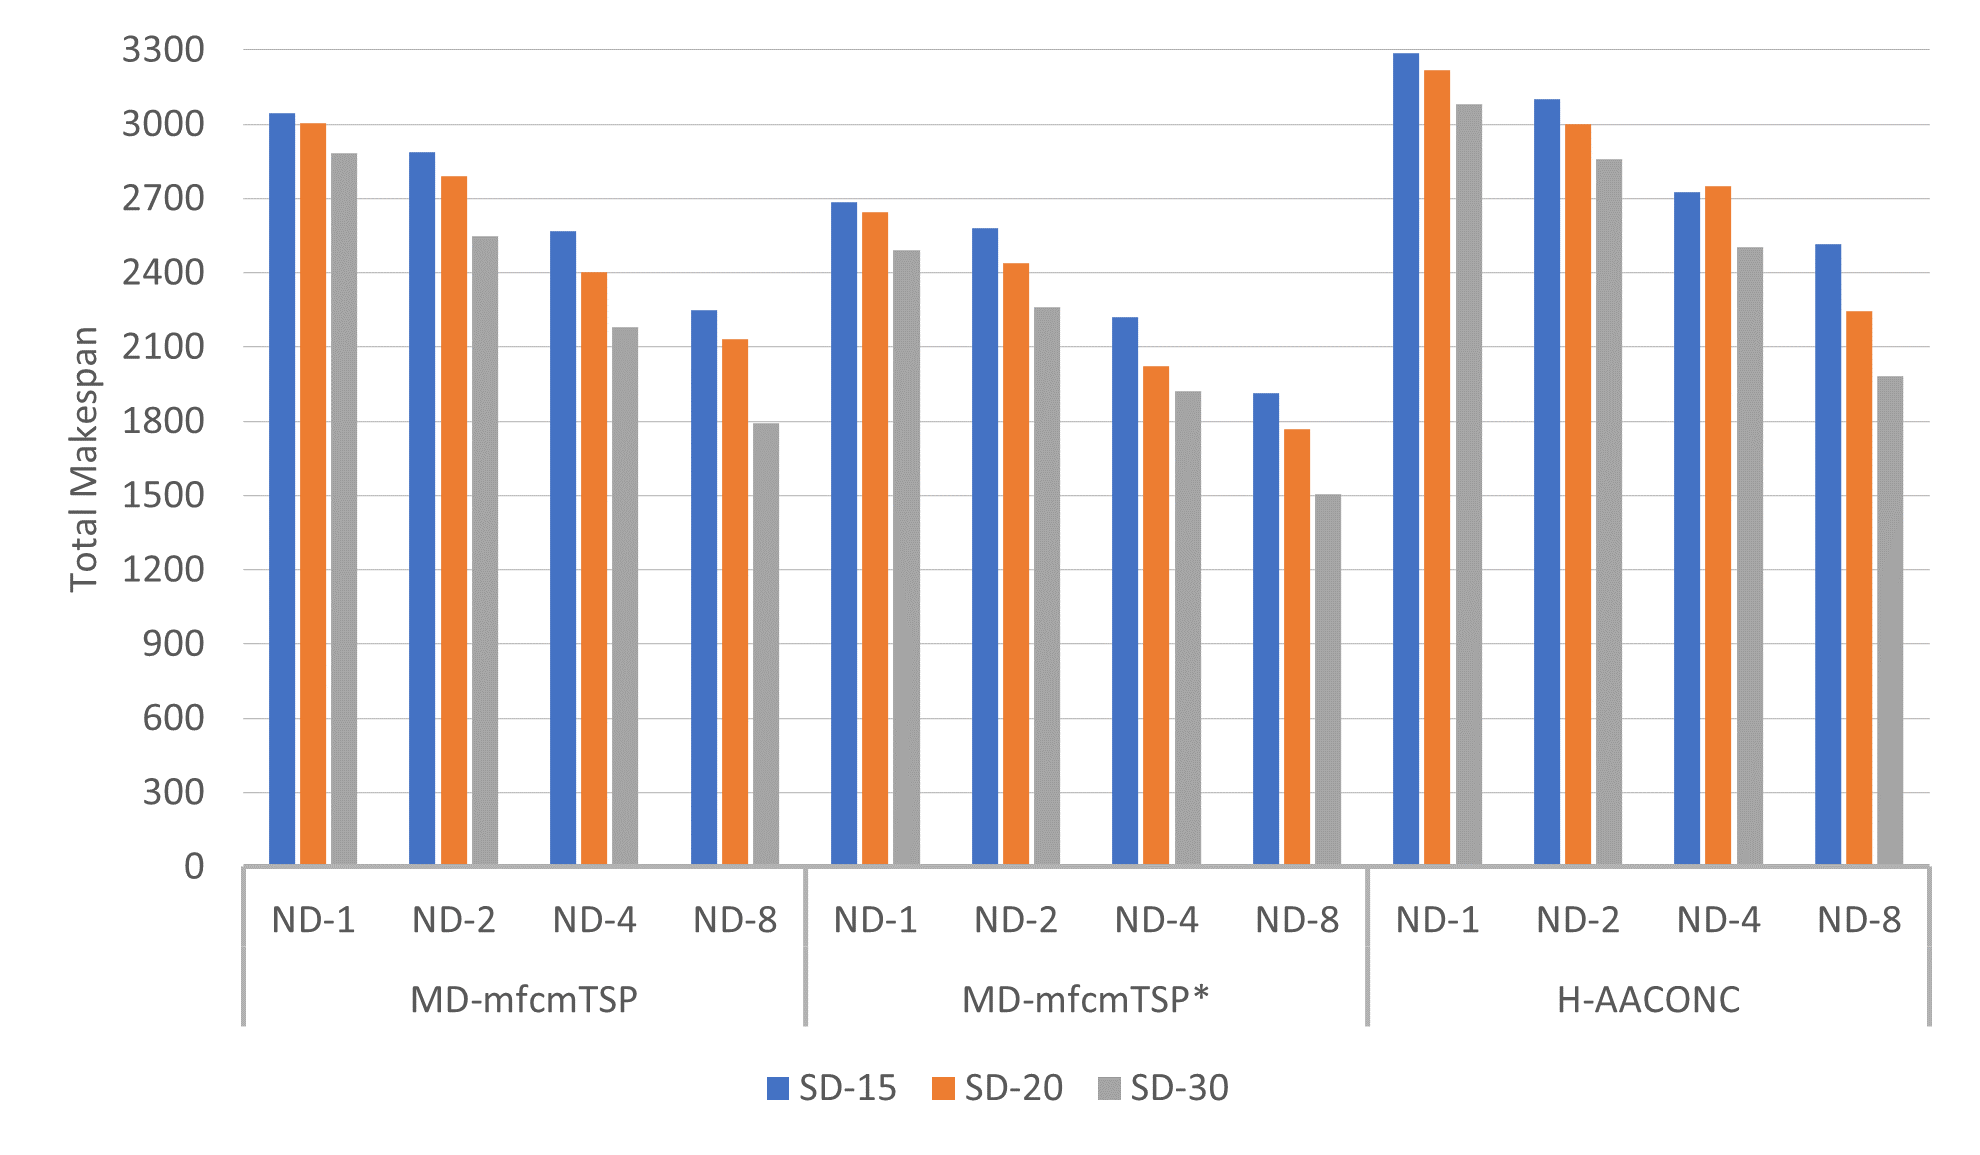
\includegraphics[scale=0.42]{p35_drones}\;
			\caption{Instance 16}
			\label{fig:p35_drones}
		\end{minipage}
	\end{figure}
	
	\begin{table}[h]
	\centering
	\caption{H-AACONC Results for $S_T=15$, $S_M=15$, $S_D=15$}
	\begin{tabular}{@{}ccccccc@{}}
		\midrule
		\textbf{Instance} & \textbf{Best} & \textbf{Average} & \textbf{Gap (\%)} & \textbf{Worst} & \textbf{Gap (\%)} & \textbf{Time (s)} \\ \midrule
		1  & 240.59 & 244.86 & 1.78 & 250.60 & 4.16 & 59   \\ \midrule
		2  & 249.29 & 267.35 & 7.25 & 297.99 & 19.54 & 55  \\ \midrule
		3  & 237.15 & 239.94 & 1.18 & 242.69 & 2.34 & 136  \\ \midrule
		4  & 720.64 & 724.97 & 0.60 & 734.08 & 1.87 & 240  \\ \midrule
		5  & 701.32 & 708.03 & 0.96 & 716.98 & 2.23 & 304  \\ \midrule
		6  & 443.93 & 451.51 & 1.71 & 461.98 & 4.07 & 296  \\ \midrule
		7  & 344.91 & 363.06 & 5.26 & 403.51 & 16.99 & 237  \\ \midrule
		8  & 3280.55 & 3354.50 & 2.25 & 3540.63 & 7.93 & 3433  \\ \midrule
		9  & 2101.33 & 2127.10 & 1.23 & 2167.92 & 3.17 & 3198  \\ \midrule
		10 & 1591.48 & 1611.05 & 1.23 & 1634.04 & 2.67 & 2986  \\ \midrule
		11 & 1215.86 & 1239.40 & 1.94 & 1268.39 & 4.32 & 2460  \\ \midrule
		12 & 1996.01 & 2040.53 & 2.23 & 2125.57 & 6.49 & 3600  \\ \midrule
		13 & 2018.11 & 2045.58 & 1.36 & 2085.06 & 3.32 & 3600  \\ \midrule
		14 & 1667.32 & 1690.26 & 1.38 & 1728.06 & 3.64 & 3600  \\ \midrule
		15 & 4551.42 & 4739.77 & 4.14 & 4917.98 & 8.05 & 3600  \\ \midrule
		16 & 3217.83 & 3286.65 & 2.14 & 3337.64 & 3.72 & 3600  \\ \midrule
	\end{tabular}
	\label{table:ACO_15-15-15}
\end{table}\;
	\begin{table}[h]
	\centering
	\caption{H-AACONC Results for speeds: $S_T=15$, $S_M=20$, $S_D=20$}
	\begin{tabular}{@{}ccccccc@{}}
		\midrule
		\textbf{Instance} & \textbf{Best} & \textbf{Average} & \textbf{Gap (\%)} & \textbf{Worst} & \textbf{Gap (\%)} & \textbf{Time (s)} \\ \midrule
		1  & 209.11 & 211.09 & 0.94 & 213.07 & 1.89 & 62   \\ \midrule
		2  & 203.21 & 211.95 & 4.30 & 217.73 & 7.15 & 59   \\ \midrule
		3  & 202.84 & 208.02 & 2.55 & 209.93 & 3.50 & 187  \\ \midrule
		4  & 644.53 & 648.42 & 0.60 & 653.55 & 1.40 & 273  \\ \midrule
		5  & 626.27 & 631.51 & 0.84 & 643.01 & 2.67 & 263  \\ \midrule
		6  & 395.97 & 405.98 & 2.53 & 415.89 & 5.03 & 272  \\ \midrule
		7  & 302.03 & 309.89 & 2.60 & 317.51 & 5.13 & 245  \\ \midrule
		8  & 2980.82 & 3044.99 & 2.15 & 3122.26 & 4.75 & 3186  \\ \midrule
		9  & 1878.13 & 1898.64 & 1.09 & 1922.72 & 2.37 & 3482  \\ \midrule
		10 & 1448.47 & 1480.76 & 2.23 & 1506.14 & 3.98 & 2661  \\ \midrule
		11 & 1114.90 & 1135.19 & 1.82 & 1148.02 & 2.97 & 2174  \\ \midrule
		12 & 1780.21 & 1818.28 & 2.14 & 1842.74 & 3.51 & 3600  \\ \midrule
		13 & 1826.29 & 1871.63 & 2.48 & 1910.65 & 4.62 & 3600  \\ \midrule
		14 & 1527.89 & 1562.78 & 2.28 & 1605.48 & 5.08 & 3600  \\ \midrule
		15 & 4391.44 & 4511.28 & 2.73 & 4593.45 & 4.60 & 3600  \\ \midrule
		16 & 3068.08 & 3111.75 & 1.42 & 3158.51 & 2.95 & 3600  \\ \midrule
	\end{tabular}
	\label{table:ACO_15-20-20}
\end{table}
\;
	\begin{table}[h]
	\centering
	\caption{H-AACONC Results for $S_T=15$, $S_M=20$, $S_D=30$}
	\begin{tabular}{@{}ccccccc@{}}
		\midrule
		\textbf{Instance} & \textbf{Best} & \textbf{Average} & \textbf{Gap (\%)} & \textbf{Worst} & \textbf{Gap (\%)} & \textbf{Time (s)} \\ \midrule
		1  & 195.35 & 195.91 & 0.28 & 196.20 & 0.44 & 61   \\ \midrule
		2  & 193.96 & 195.05 & 0.56 & 196.48 & 1.30 & 63 \\ \midrule
		3  & 181.59 & 189.27 & 4.23 & 197.05 & 8.51 & 136 \\ \midrule
		4  & 595.11 & 603.03 & 1.33 & 608.86 & 2.31 & 263 \\ \midrule
		5  & 593.05 & 601.47 & 1.42 & 614.37 & 3.59 & 327 \\ \midrule
		6  & 373.69 & 379.01 & 1.42 & 385.79 & 3.24 & 216 \\ \midrule
		7  & 289.75 & 295.56 & 2.00 & 301.55 & 4.07 & 229 \\ \midrule
		8  & 2801.15 & 2854.09 & 1.89 & 2892.70 & 3.27 & 3454 \\ \midrule
		9  & 1765.80 & 1789.67 & 1.35 & 1824.08 & 3.30 & 3325 \\ \midrule
		10 & 1341.89 & 1392.54 & 3.77 & 1483.68 & 10.57 & 2161 \\ \midrule
		11 & 1035.50 & 1049.95 & 1.40 & 1072.10 & 3.53 & 2929 \\ \midrule
		12 & 1723.00 & 1751.76 & 1.67 & 1789.12 & 3.84 & 3600 \\ \midrule
		13 & 1753.06 & 1784.82 & 1.81 & 1810.94 & 3.30 & 3600 \\ \midrule
		14 & 1438.99 & 1477.18 & 2.65 & 1493.71 & 3.80 & 3600 \\ \midrule
		15 & 4250.11 & 4369.42 & 2.81 & 4449.05 & 4.68 & 3600 \\ \midrule
		16 & 2994.14 & 3013.30 & 0.64 & 3052.88 & 1.96 & 3600 \\ \midrule
	\end{tabular}
	\label{table:ACO_15-20-30}
\end{table}
\;
	
	\clearpage
	\printbibliography
	
\end{document}
